\documentclass[UTF8,a4paper,zihao=5,fontset=fandol]{ctexart}
    \usepackage[margin=21mm,headheight=15pt]{geometry}
    \usepackage{amsmath,amssymb,bm,graphicx,longtable,booktabs,array,enumitem,fvextra,xcolor,xurl,fancyhdr,needspace}
    \usepackage{hyperref}
    \setmainfont{DejaVu Serif}
    \setsansfont{DejaVu Sans}
    \setmonofont[Scale=.88]{DejaVu Sans Mono}
    \definecolor{bluegray}{HTML}{285B7A}
    \hypersetup{colorlinks=true,linkcolor=bluegray,urlcolor=bluegray,pdftitle={EM500核力与两核子态求解},pdfauthor={含时量子多体调研项目}}
    \setlength{\parindent}{0pt}
    \setlength{\parskip}{.5em}
    \setlength{\emergencystretch}{3em}
    \setlist{nosep,leftmargin=2em}
    \setcounter{tocdepth}{2}
    \renewcommand{\baselinestretch}{1.14}
    \pagestyle{fancy}\fancyhf{}
    \fancyhead[L]{\small EM500核力与两核子态求解}
    \fancyhead[R]{\small v0.3 / code v0.5.2}
    \fancyfoot[C]{\thepage}
    \newsavebox{\EquationBox}
    \newcommand{\FitEquation}[1]{\sbox{\EquationBox}{$\displaystyle #1$}%
    \ifdim\wd\EquationBox>.92\linewidth\resizebox{.92\linewidth}{!}{\usebox{\EquationBox}}\else\usebox{\EquationBox}\fi}
    \allowdisplaybreaks
    \begin{document}
    \begin{titlepage}\centering\vspace*{28mm}
{\Huge\bfseries EM500核力与两核子态求解\par}\vspace{12mm}
{\Large 程序说明书与操作教程\par}\vspace{8mm}
{\large 文档 v0.3 · 代码 v0.5.2\par}\vspace{8mm}
2026年9月30日\vfill
\begin{minipage}{.86\textwidth}\large
从物理模型、连续方程与离散求解，到源码、输入和结果。\par\medskip
包含氘核、np散射、pp散射三个逐步操作范例。\end{minipage}\vspace*{20mm}\end{titlepage}
\tableofcontents\clearpage
程序说明书与操作教程 · 文档 v0.3 · 对应代码 v0.5.2 · 2026年9月30日

本书介绍公开发布包中的 Fortran 程序，包括所采用的 EM500 核力、氘核束缚态与 np、pp 弹性散射的求解方法，以及输入设置和结果分析。阅读所需的基础知识包括波函数、薛定谔方程和矩阵乘法；主值积分、分波通道和散射矩阵等概念将在相应章节中介绍。

首次使用程序时，可先读第1、2章了解计算任务和物理模型，再按第7章完成三个操作范例。第3—5章依次介绍氘核、np 散射和 pp 散射，均按照物理问题、连续方程、数值方程、源码与输出的顺序展开。第6章介绍代码结构，第8章介绍数值精度检查，第9章讨论实验比较。附录汇总符号约定、接口和输入输出，供查阅使用。

文中路径除特别说明外均相对于公开发布包的根目录，即包含 {\ttfamily\small Makefile}、{\ttfamily\small run.\allowbreak{}sh} 和 {\ttfamily\small app/\allowbreak{}} 的目录。本书的计算范围为两核子体系：氘核束缚态、np 弹性散射和 pp 弹性散射。公开版保留模型、求解器、科学数据与自制图，COUL90特殊函数源码按第7.1节在首次构建时获取并校验。范例运行记录的来源及分发说明见附录D。

\clearpage\section*{第1章 计算任务与结果}\addcontentsline{toc}{section}{第1章 计算任务与结果}
\Needspace{6\baselineskip}\subsection*{1.1 三个问题共用一套核力}\addcontentsline{toc}{subsection}{1.1 三个问题共用一套核力}
氘核是一个质子和一个中子的束缚态。其相对运动的能量小于分离后的两核子能量；计算要找出这个负本征值及其波函数。np 散射仍然是一个质子和一个中子，但能量为正，并指定了入射状态。pp 散射则有两个相同质子，需要同时处理核相互作用、库仑相互作用和交换反对称性。


{\small\setlength{\tabcolsep}{3pt}\renewcommand{\arraystretch}{1.28}
\begin{longtable}{@{}>{\raggedright\arraybackslash}p{0.235\linewidth}>{\raggedright\arraybackslash}p{0.235\linewidth}>{\raggedright\arraybackslash}p{0.235\linewidth}>{\raggedright\arraybackslash}p{0.235\linewidth}@{}}\toprule
\textbf{任务} & \textbf{已知输入} & \textbf{主要待求量} & \textbf{可与实验联系的结果}\\\midrule
\endfirsthead
\textbf{任务} & \textbf{已知输入} & \textbf{主要待求量} & \textbf{可与实验联系的结果}\\\midrule
\endhead
氘核 & EM500、体系量子数 & 束缚能与 S/D 波函数 & 结合能、半径及电磁观测量的近似值\\
np 弹性散射 & EM500、入射能量 & 各分波散射矩阵 & 角分布、积分弹性截面、相移\\
pp 弹性散射 & pp 核力、库仑、入射能量 & 库仑背景下的核散射矩阵 & 两质子弹性角分布\\
\bottomrule\end{longtable}}
三个任务使用固定的核力及其配套参数，先求解量子力学方程，再由解计算观测量。不同入射能量下的散射曲线使用同一套参数，所得结果与相应实验数据比较。

\Needspace{6\baselineskip}\subsection*{1.2 从输入到归档}\addcontentsline{toc}{subsection}{1.2 从输入到归档}
整个计算顺序可以写成：


\begin{Verbatim}[samepage=true,breaklines=true,breakanywhere=true,fontsize=\small,frame=leftline,framesep=3mm,rulecolor=\color{bluegray}]
根目录的输入文件
  -> fewbody：读取、验证输入，选择任务
  -> EM500接口：提供给定通道与动量的势矩阵元
  -> 氘核：解矩阵本征问题 -> 波函数 -> 能量/半径等
     np：解主值积分方程 -> K/T/S -> 振幅 -> 截面
     pp：解截断库仑问题 -> 外区匹配 -> 振幅 -> 截面
  -> 根目录写结果、日志、实际输入快照
  -> 成功结束：按完成时刻归档到 output/
\end{Verbatim}
核力调用、方程求解和观测量计算均由 Fortran 程序实现。部分绘图程序采用 Python，读取计算结果并生成图表。服务器运行所需的编译和执行步骤见第7章。

\Needspace{6\baselineskip}\subsection*{1.3 结果的三个层次}\addcontentsline{toc}{subsection}{1.3 结果的三个层次}
\textbf{模型层次}确定计算所采用的相互作用、电磁算符和反应通道。\textbf{数值层次}涉及方程的求解精度，由动量节点数、积分上限、角动量截断等设置控制。\textbf{实验比较层次}涉及观测量的定义，包括入射能量、角度参考系、出射粒子、单位及实验接受度。

这三个层次分别对应不同的检查。例如，增加动量节点用于检查积分的数值精度；选择电磁算符决定半径和电磁矩的计算近似；比较实验时还需核对能量和观测量定义。第8、9章将分别介绍这些检查。

\clearpage\section*{第2章 物理模型与基本约定}\addcontentsline{toc}{section}{第2章 物理模型与基本约定}
\Needspace{6\baselineskip}\subsection*{2.1 核力是一种势能算符}\addcontentsline{toc}{subsection}{2.1 核力是一种势能算符}
本程序中的“核力”指薛定谔方程里的势能算符 \(V\)，它作用于两核子相对运动的波函数。相互作用取决于核子的自旋、同位旋及相对运动，因此核力的描述包含空间、自旋和动量等多种结构。可从以下三个层次理解这些结构。


{\small\setlength{\tabcolsep}{3pt}\renewcommand{\arraystretch}{1.28}
\begin{longtable}{@{}>{\raggedright\arraybackslash}p{0.2784\linewidth}>{\raggedright\arraybackslash}p{0.3264\linewidth}>{\raggedright\arraybackslash}p{0.3552\linewidth}@{}}\toprule
\textbf{分类层次} & \textbf{名称} & \textbf{物理含义}\\\midrule
\endfirsthead
\textbf{分类层次} & \textbf{名称} & \textbf{物理含义}\\\midrule
\endhead
算符结构 & 中心、自旋—自旋、张量、自旋—轨道 & 规定空间、自旋与角动量怎样耦合\\
物理机制 & 单π交换、双π交换、接触项 & 区分长程、中程和未显式分辨的短程贡献\\
数学表示 & 坐标/动量表示，局域/非局域，分波 & 规定算符的表示和求解方式\\
\bottomrule\end{longtable}}
表中三个层次分别说明算符结构、物理机制和数学表示。它们之间相互联系：单π交换可以同时产生自旋—自旋和张量结构；多个结构的系数都可以依赖动量。张量作用使氘核的 S 波与 D 波相互耦合，两者分别对应轨道角动量 \(L=0\) 和 \(L=2\)。

在坐标表示中，局域势通过 \(V(\boldsymbol r)\psi(\boldsymbol r)\) 作用于波函数；非局域势则通过积分联系不同位置的波函数分量。本程序在动量表示下求解方程，所需的势矩阵元为


\begin{equation*}\FitEquation{V_{L'L}^{JS T_{\rm iso}}(p',p)
=\langle p',L';JS T_{\rm iso}|V|p,L;JS T_{\rm iso}\rangle .}\tag{2.1}\end{equation*}


第一组指标 \((L',p')\) 标记输出态，第二组 \((L,p)\) 标记输入态。势矩阵元给出势能算符对这些状态分量的耦合。求解时，对输入动量积分，并对允许的轨道通道求和，即可得到算符作用后的波函数分量；第3、4章将写出具体方程。

\Needspace{6\baselineskip}\subsection*{2.2 从手征框架到 EM500}\addcontentsline{toc}{subsection}{2.2 从手征框架到 EM500}
手征有效场论以核子和π介子等低能自由度描述强相互作用，继承 QCD 的低能对称性及其破缺方式。对称性约束可出现的相互作用结构；各项强度由相应的耦合常数决定，其中的待定系数通过实验数据约束。它把相互作用按低动量阶次组织，使逐阶改进和估计截断误差成为可能。\href{https://arxiv.org/abs/1105.2919}{手征核力综述}

LO（leading order）表示领先阶，NLO、N²LO、N³LO 表示依次更高的阶次。在这里采用的计数中，它们分别对应动量计数的 0、2、3、4 阶。N³LO 势包含从 LO 到 N³LO 的全部保留项；阶次表示相互作用展开的精细程度。

本程序的 EM500 指 \textbf{Entem–Machleidt 2003 Idaho N³LO 两核子势的 500 MeV 版本}。它是手征核力框架下的一套具体势，由特定的构造方案、调节器和配套参数共同确定。\href{https://arxiv.org/abs/nucl-th/0304018}{原始构造论文}

EM500 核力的 Fortran 源文件取自 Tic-tac 公开代码，原样保存在 {\ttfamily\small app/\allowbreak{}em500/\allowbreak{}}。本项目编写了调用接口、氘核与散射求解器，以及观测量计算程序。第6章介绍各部分的职责，第8章说明源码一致性和求解结果的检验方法。

\Needspace{6\baselineskip}\subsection*{2.3 常数、接触系数与拟合范围}\addcontentsline{toc}{subsection}{2.3 常数、接触系数与拟合范围}
程序以 35 个数保存核力配置，包括接触系数、轴矢耦合及πN低能常数等。这组输入汇集了预先确定的常数和拟合得到的系数。数值在 {\ttfamily\small app/\allowbreak{}em500\_\allowbreak{}parameters.\allowbreak{}f90}，名称、历史质量和单位约定在 {\ttfamily\small app/\allowbreak{}provenance/\allowbreak{}em500.\allowbreak{}json}。


{\small\setlength{\tabcolsep}{3pt}\renewcommand{\arraystretch}{1.28}
\begin{longtable}{@{}>{\raggedright\arraybackslash}p{0.2784\linewidth}>{\raggedright\arraybackslash}p{0.3264\linewidth}>{\raggedright\arraybackslash}p{0.3552\linewidth}@{}}\toprule
\textbf{类别} & \textbf{例子} & \textbf{在本程序中的处理}\\\midrule
\endfirsthead
\textbf{类别} & \textbf{例子} & \textbf{在本程序中的处理}\\\midrule
\endhead
历史质量和耦合常数 & 核子/π质量、\(F_\pi,g_A\) & 沿用固定势的取值\\
πN低能常数 & \(c_i,d_i\) 的组合 & 进入π交换部分，采用配套配置\\
NN接触系数 & \(\widetilde C,C,D\) & 描述未显式分辨的短程作用，采用固定配套系数\\
调节方案 & \(\Lambda,n\) & 与参数共同定义当前势\\
\bottomrule\end{longtable}}
原构造用相移帮助确定参数，并拟合两核子散射数据；报告的数据库能区为实验室动能低于 290 MeV。氘核结合能也是定参约束之一，因而适合作为核力调用和束缚态求解的检验量。本书还给出 300.2 MeV 的散射比较，作为原报告拟合能区之外的检验。

\Needspace{6\baselineskip}\subsection*{2.4 分项与调节器}\addcontentsline{toc}{subsection}{2.4 分项与调节器}
从机制看，固定势由π交换、不同阶接触项以及实现中指定的电荷依赖等修正组成。每一项再投影到式(2.1)的分波基，得到求解器需要的矩阵元。完整表达式可参照 EM 综述及原构造论文。本程序调用所附的固定核力源码，直接获得这些分波矩阵元。

常见调节函数为


\begin{equation*}\FitEquation{f_n(p',p)=\exp\left[-(p'/\Lambda)^{2n}-(p/\Lambda)^{2n}\right],
\qquad\Lambda=500\ {\rm MeV}/c .}\tag{2.2}\end{equation*}


调节函数随动量增加而平滑减小，从而抑制高动量贡献；高于 500 MeV/c 的部分仍包含在积分中，其权重由调节函数控制。不同分项可以采用不同指数：当前预设单π取 \(n=4\)、双π取 \(n=2\)，接触项依通道、阶次采用各自规则。这些设置由 {\ttfamily\small chp-set.\allowbreak{}f90} 给出，核力接口返回的势矩阵元已包含相应调节因子。


{\small\setlength{\tabcolsep}{3pt}\renewcommand{\arraystretch}{1.28}
\begin{longtable}{@{}>{\raggedright\arraybackslash}p{0.2784\linewidth}>{\raggedright\arraybackslash}p{0.3264\linewidth}>{\raggedright\arraybackslash}p{0.3552\linewidth}@{}}\toprule
\textbf{数字或输入} & \textbf{作用对象} & \textbf{含义}\\\midrule
\endfirsthead
\textbf{数字或输入} & \textbf{作用对象} & \textbf{含义}\\\midrule
\endhead
290 MeV & 入射实验室动能 & 原报告拟合范围的上限\\
500 MeV/c & 相对动量 & EM500 固定调节尺度\\
{\ttfamily\small pmax\_\allowbreak{}MeV=\allowbreak{}1000} & 数值积分变量 & 当前求积区间的上端\\
{\ttfamily\small n\_\allowbreak{}grid=\allowbreak{}96} 等 & 求积节点 & 在给定区间内近似积分的分辨率\\
\bottomrule\end{longtable}}
改变后两项用于检查数值求解；改变调节器或核力参数通常意味着改变物理模型。接触系数的使用还涉及单位缩放，本程序沿用原核力源码中的换算方式，使参数、动量和势矩阵元采用一致的单位约定。

\Needspace{6\baselineskip}\subsection*{2.5 相对运动、单位与指标}\addcontentsline{toc}{subsection}{2.5 相对运动、单位与指标}
令 \(\boldsymbol r=\boldsymbol r_n-\boldsymbol r_p\)，\(p\) 为其共轭相对动量大小。分离质心后，np 相对动能为


\begin{equation*}\FitEquation{H_0=\frac{p^2}{2\mu}=\frac{p^2}{m},\qquad
\mu=\frac{M_nM_p}{M_n+M_p},\quad m=2\mu .}\tag{2.3}\end{equation*}


代码取 \(M_p=938.272\) MeV、\(M_n=939.5653\) MeV，故 \(m=938.9182046406256\) MeV，\(\hbar c=197.327\) MeV fm。这里使用 \(c=1\)，但从动量转到 fm 时明确保留 \(\hbar c\)。pp 的相对质量参数为 \(m=M_p\)。电荷半径后处理另用相应的电磁常数；核力计算仍沿用上述历史常数。


{\small\setlength{\tabcolsep}{3pt}\renewcommand{\arraystretch}{1.28}
\begin{longtable}{@{}>{\raggedright\arraybackslash}p{0.3705\linewidth}>{\raggedright\arraybackslash}p{0.6045\linewidth}@{}}\toprule
\textbf{符号/名称} & \textbf{含义}\\\midrule
\endfirsthead
\textbf{符号/名称} & \textbf{含义}\\\midrule
\endhead
\(p,p',k_i\) & 方程中的相对动量；\(k_i\) 是积分节点\\
\(q\) & 给定入射能量对应的在壳相对动量\\
\(L,S,J\) & 相对轨道角动量、两核子总自旋、总角动量\\
\(T_{\rm iso}\) & 同位旋；与散射矩阵 \(T\) 区分\\
\(a,b\) & 一个固定分波块内部的通道编号\\
\(i,j\) & 动量网格节点的编号\\
\(N\)、{\ttfamily\small n\_\allowbreak{}grid} & 每个轨道通道的动量节点数\\
\bottomrule\end{longtable}}
自旋 \(S=0,1\)，谱项写作 \({}^{2S+1}L_J\)。例如 \({}^3S_1\) 的大写字母 S 表示 \(L=0\)，左上角 3 则表示总自旋为 1。一个耦合块有两个轨道通道，Fortran 数组 {\ttfamily\small ls(1),ls(2)} 分别保存第1、2个通道的轨道角动量 \(L\)。

\Needspace{6\baselineskip}\subsection*{2.6 适用范围与模型近似}\addcontentsline{toc}{subsection}{2.6 适用范围与模型近似}
本程序面向两核子体系，使用固定的两核子相互作用。散射计算采用实势下的弹性模型。介子产生等非弹性通道在当前模型范围之外；接近或超过相应阈值时，比较实验需要考虑这些通道的影响。

核力按原实现的预设包含部分相对论修正及 minimal-relativity 归一化；Kamada–Glöckle 变换处于关闭状态。入射动量采用精确运动学换算，传播子则采用式(2.3)的非相对论形式。这些约定共同确定了当前求解模型。pp 的库仑处理及其运动学约定见第5章，氘核电磁观测量的算符近似见第3章。

具体能区内的适用性需要结合核力的拟合范围、模型近似和实验比较来评估，第9章给出相应实例。

\clearpage\section*{第3章 氘核束缚态的计算}\addcontentsline{toc}{section}{第3章 氘核束缚态的计算}
\Needspace{6\baselineskip}\subsection*{3.1 相对运动与两个径向分量}\addcontentsline{toc}{subsection}{3.1 相对运动与两个径向分量}
分离质心运动后，氘核的待求量是中子与质子的相对运动波函数。令相对动量为 \(p\)，约化质量为 \(\mu=M_nM_p/(M_n+M_p)\)。程序使用 \(m=2\mu=938.9182046406256\ \mathrm{MeV}\)，将动能写为 \(p^2/m\)。这里采用 \(c=1\) 的单位制；转换到 fm 时显式保留 \(\hbar c=197.327\ \mathrm{MeV\,fm}\)。

氘核基态的量子数为 \(J=1\)、正宇称、自旋 \(S=1\)、同位旋 \(T=0\)。相应的轨道角动量为 \(L=0,2\)，即 \({}^3S_1\) 与 \({}^3D_1\) 通道。张量力将这两个通道耦合，相对运动因而归结为两个径向分量 \(\psi_0(p)\) 与 \(\psi_2(p)\) 的耦合问题。程序按 S、D 波的顺序将它们编号为第1、2通道。

这两个径向分量满足耦合薛定谔方程：


\begin{equation*}\FitEquation{\frac{p^2}{m}\psi_L(p)+\sum_{L'=0,2}\int_0^\infty dp'\,p'^2V_{LL'}(p,p')\psi_{L'}(p')=E_d\psi_L(p),\qquad L=0,2.}\tag{3.1}\end{equation*}


\(V_{LL'}(p,p')\) 是从输入分量 \((L',p')\) 到输出分量 \((L,p)\) 的势核，由固定参数的 EM500 源码提供。程序采用积分测度 \(dp'\,p'^2\)，势核单位为 \(\mathrm{MeV}^{-2}\)；相应的归一化因子已包含在势核定义中，方程采用式（3.1）所示形式。束缚态能量 \(E_d<0\)，结合能定义为 \(B_d=-E_d>0\)。波函数满足归一化条件：


\begin{equation*}\FitEquation{\int_0^\infty dp\,p^2[\psi_0(p)^2+\psi_2(p)^2]=1.}\tag{3.2}\end{equation*}


\Needspace{6\baselineskip}\subsection*{3.2 从积分方程到对称矩阵}\addcontentsline{toc}{subsection}{3.2 从积分方程到对称矩阵}
数值计算将积分上限取为 \(P=\texttt{pmax\_MeV}\)，在 \((0,P)\) 上使用 \(N=\texttt{n\_grid}\) 个 Gauss–Legendre 求积点。\(p_i\) 是动量节点，\(w_i\) 是对应的积分权重，两者都具有 MeV 单位。节点按非均匀间距分布，各节点的积分贡献由相应权重确定：


\begin{equation*}\FitEquation{\int_0^P F(p)dp\simeq\sum_{i=1}^Nw_iF(p_i),\qquad
\frac{p_i^2}{m}\psi_L(p_i)+\sum_{L'j}w_jp_j^2V_{LL'}(p_i,p_j)\psi_{L'}(p_j)=E_d\psi_L(p_i).}\tag{3.3}\end{equation*}


式（3.3）的积分权重随输入列的节点变化。为将离散方程写成实对称矩阵的本征值问题，定义无量纲变量 \(y_{Li}=f_i\psi_L(p_i)\)，其中 \(f_i=p_i\sqrt{w_i}\)，得到


\begin{equation*}\FitEquation{H_{Li,L'j}=\delta_{LL'}\delta_{ij}\frac{p_i^2}{m}+f_iV_{LL'}(p_i,p_j)f_j,\qquad Hy=E_dy.}\tag{3.4}\end{equation*}


矩阵维数为 \(2N\times2N\)，前 \(N\) 个分量对应 S 波，后 \(N\) 个对应 D 波。程序分别计算两个动量次序的势核，先检查势核的互易性，再检查 \(H\) 的对称性。检查通过后，对浮点舍入造成的微小不对称作对称化处理。

{\ttfamily\small solve\_\allowbreak{}deuteron} 调用 LAPACK 的 {\ttfamily\small DSYEV} 求本征值和本征矢，并选取最低负本征值及其本征矢作为氘核束缚态解。同一离散矩阵的正本征值给出连续谱在有限离散空间中的表示。

\Needspace{6\baselineskip}\subsection*{3.3 波函数恢复与代码对应}\addcontentsline{toc}{subsection}{3.3 波函数恢复与代码对应}
由加权本征矢恢复动量波函数，并计算归一化、D态概率和矩阵残差：


\begin{equation*}\FitEquation{\psi_L(p_i)=\frac{y_{Li}}{p_i\sqrt{w_i}},\quad
\sum_{Li}y_{Li}^2=1,\quad P_D=\sum_i y_{2i}^2,\quad
\epsilon_H=\|Hy-E_dy\|_2.}\tag{3.5}\end{equation*}


矩阵残差 \(\epsilon_H\) 衡量当前本征方程的求解精度；改变 \(N\)、\(P\) 后的结果稳定性衡量连续问题的离散误差。这两项检查分别覆盖线性代数求解和数值离散两个环节。\(P_D\) 给出当前相互作用及表示下的 D 波成分，是依赖模型与表示的诊断量。


{\small\setlength{\tabcolsep}{3pt}\renewcommand{\arraystretch}{1.28}
\begin{longtable}{@{}>{\raggedright\arraybackslash}p{0.2784\linewidth}>{\raggedright\arraybackslash}p{0.3264\linewidth}>{\raggedright\arraybackslash}p{0.3552\linewidth}@{}}\toprule
\textbf{物理量} & \textbf{实际代码变量} & \textbf{形状与含义}\\\midrule
\endfirsthead
\textbf{物理量} & \textbf{实际代码变量} & \textbf{形状与含义}\\\midrule
\endhead
\(p_i,w_i\) & {\ttfamily\small result\%p}, {\ttfamily\small result\%w} & 各 \(N\) 个元素\\
\(V_{LL'}(p_i,p_j)\) & {\ttfamily\small result\%potential\_\allowbreak{}kernel} & \(2N\times2N\)，未乘积分权重\\
\(H,y\) & {\ttfamily\small result\%hamiltonian}, {\ttfamily\small result\%weighted\_\allowbreak{}eigenvector} & \(2N\times2N\)、\(2N\)\\
\(\psi_0,\psi_2\) & {\ttfamily\small result\%psi\_\allowbreak{}s}, {\ttfamily\small result\%psi\_\allowbreak{}d} & 各 \(N\) 个动量波函数值\\
\(E_d,B_d,\epsilon_H\) & {\ttfamily\small energy\_\allowbreak{}MeV}, {\ttfamily\small binding\_\allowbreak{}MeV}, {\ttfamily\small residual\_\allowbreak{}MeV} & {\ttfamily\small deuteron\_\allowbreak{}result} 的标量成员\\
\bottomrule\end{longtable}}
上述求解由 {\ttfamily\small app/\allowbreak{}deuteron\_\allowbreak{}solver.\allowbreak{}f90} 实现。{\ttfamily\small app/\allowbreak{}em500\_\allowbreak{}force.\allowbreak{}f90} 的 {\ttfamily\small sd\_\allowbreak{}kernel(pout,pin,block)} 提供 \(2\times2\) 势块，行对应输出通道，列对应输入通道。{\ttfamily\small app/\allowbreak{}fewbody.\allowbreak{}f90} 将能量与诊断写入 {\ttfamily\small deuteron\_\allowbreak{}summary.\allowbreak{}txt}，将波函数写入 {\ttfamily\small deuteron\_\allowbreak{}wavefunction.\allowbreak{}csv}。该 CSV 同时保存动量空间的约化函数 \(p\psi_L(p)\)；下一节定义经积分变换得到的坐标空间径向函数。

\Needspace{6\baselineskip}\subsection*{3.4 坐标波函数、密度与半径}\addcontentsline{toc}{subsection}{3.4 坐标波函数、密度与半径}
动量空间的解可通过积分变换表示为中子—质子间距 \(r\) 的函数。定义坐标空间的约化径向函数 \(u(r)=u_0(r)\)、\(w(r)=u_2(r)\)：


\begin{equation*}\FitEquation{u_L(r)=\sqrt{\frac2\pi}\frac{r}{(\hbar c)^{3/2}}
\int_0^\infty dp\,p^2 j_L\!\left(\frac{pr}{\hbar c}\right)\psi_L(p).}\tag{3.6}\end{equation*}


\(j_L\) 为球 Bessel 函数，\(u,w\) 的单位为 \(\mathrm{fm}^{-1/2}\)。程序在原动量网格上以求积和计算变换，再在均匀坐标网格上用复合 Simpson 公式积分。按照原核力的 {\ttfamily\small radial\_\allowbreak{}rephased} 相位约定，S、D 两个分量都采用式（3.6）中的正号。

\(P(r)=u(r)^2+w(r)^2\) 是按径向长度定义的相对间距概率密度，\(P(r)dr\) 表示间距落在 \([r,r+dr]\) 内的概率。核子的空间密度则按体积定义。程序采用标准等质量质心几何，以 \(R=r/2\) 表示单核子距质心的距离，输出未极化氘核的球平均点密度：


\begin{equation*}\FitEquation{\rho_1(R)=\frac{P(2R)}{2\pi R^2},\qquad \rho_N(R)=2\rho_1(R),\qquad
r_{\rm pt}^2=\frac14\int_0^\infty dr\,r^2P(r).}\tag{3.7}\end{equation*}


\(\rho_1\) 的体积分为1，\(\rho_N\) 的体积分为2；\(r_{\rm pt}\) 是点核子均方根半径。等质量约定用于这里的空间几何关系，动力学求解使用实际 np 约化质量。与实验电荷半径对应的理论值还需计入核子自身的电荷结构，具体估计式见第3.5节。

{\ttfamily\small app/\allowbreak{}deuteron\_\allowbreak{}observables.\allowbreak{}f90} 保存坐标数组 {\ttfamily\small obs\%r} 和径向波函数数组 {\ttfamily\small obs\%u}、{\ttfamily\small obs\%w}。其中 {\ttfamily\small obs\%w} 表示 D 波径向函数，动量求积权重则保存在 {\ttfamily\small result\%w}。设置 {\ttfamily\small write\_\allowbreak{}coordinate=\allowbreak{}.\allowbreak{}true.\allowbreak{}} 后，程序生成 {\ttfamily\small deuteron\_\allowbreak{}coordinate\_\allowbreak{}wavefunction.\allowbreak{}csv} 和 {\ttfamily\small deuteron\_\allowbreak{}observables.\allowbreak{}dat}。坐标波函数沿用动量空间解确定的归一化；有限坐标区间上的归一化积分偏差用于检查积分变换误差和尾部截断效应。

\Needspace{6\baselineskip}\subsection*{3.5 其他已实现的氘核量}\addcontentsline{toc}{subsection}{3.5 其他已实现的氘核量}
在单体脉冲近似下，电四极矩与磁矩由波函数给出；计入核子有限尺寸后，可进一步估计电荷半径：


\begin{equation*}\FitEquation{Q_{\rm IA}=\frac1{20}\int dr\,r^2w(\sqrt8u-w),\qquad
\mu_{\rm IA}=\mu_p+\mu_n-\frac32P_D(\mu_p+\mu_n-\tfrac12),}\tag{3.8}\end{equation*}



\begin{equation*}\FitEquation{r_{\rm ch,est}^2=r_{\rm pt}^2+r_p^2+\langle r_n^2\rangle+
\frac34\left(\frac{\hbar c}{M_p}\right)^2.}\tag{3.9}\end{equation*}


\(\mu_p,\mu_n\) 以核磁子为单位；\(r_p\) 与 \(\langle r_n^2\rangle\) 是后处理使用的核子电荷结构常数，数值均记录在输出中。式（3.8）、（3.9）采用上述算符近似，完整的两体电磁作用属于进一步扩展的内容。与实验比较时，需同时考察核力所决定的波函数和所用电磁算符。

波函数的长距离行为由渐近形式描述：


\begin{equation*}\FitEquation{u(r)\simeq A_Se^{-\gamma r},\quad
w(r)\simeq A_De^{-\gamma r}\left[1+\frac3{\gamma r}+\frac3{(\gamma r)^2}\right],\quad
\gamma=\frac{\sqrt{mB_d}}{\hbar c},\quad\eta=A_D/A_S}\tag{3.10}\end{equation*}


程序用式（3.10）提取渐近参数，在20—25 fm窗口内固定 \(\gamma\)，对 \(A_S,A_D\) 作线性最小二乘拟合。{\ttfamily\small tail\_\allowbreak{}fit\_\allowbreak{}available} 标记坐标范围是否满足拟合要求及结果是否有效。氘核计算由此形成完整流程：核力 → 束缚态矩阵 → 能量与波函数 → 指定观测算符的期望值。

\clearpage\section*{第4章 np散射的计算}\addcontentsline{toc}{section}{第4章 np散射的计算}
\Needspace{6\baselineskip}\subsection*{4.1 散射边界与在壳动量}\addcontentsline{toc}{subsection}{4.1 散射边界与在壳动量}
np散射求解 \((H_0+V)\Psi=E\Psi\) 的正能量解。远处的波函数由入射平面波和向外传播的散射球面波组成。以入射自旋态 \(\chi_\nu\) 为例：


\begin{equation*}\FitEquation{\Psi_\nu^{(+)}(\mathbf r)\underset{r\to\infty}{\sim}
e^{ikz}\chi_\nu+\frac{e^{ikr}}r\sum_{\nu\prime}f_{\nu\prime\nu}(\theta,\phi)\chi_{\nu\prime},
\qquad k=q/(\hbar c).}\tag{4.1}\end{equation*}


\(q\) 是给定入射能量对应的质心相对动量，称为在壳动量；积分方程中的其他动量是内部积分变量。入射平面波可展开为多个轨道角动量 \(L\) 的分波。未极化散射的观测量还需对入射自旋状态取平均。

本程序采用中子入射、质子靶静止的实验室动能。相对论与非相对论运动学选项分别采用以下能量—动量换算：


\begin{equation*}\FitEquation{q^2=\frac{M_p^2E_{\rm lab}(E_{\rm lab}+2M_n)}{(M_p+M_n)^2+2M_pE_{\rm lab}};
\quad\text{非相对论选项：}\quad
q^2=\frac{mM_p}{M_n+M_p}E_{\rm lab}.}\tag{4.2}\end{equation*}


两种运动学选项均将所得 \(q\) 代入 \(E=q^2/m\)，作为积分方程的能量参数。{\ttfamily\small relativistic} 指定相对论入射运动学，后续动力学计算采用本文的非相对论两体积分方程。

\Needspace{6\baselineskip}\subsection*{4.2 从薛定谔方程到K矩阵}\addcontentsline{toc}{subsection}{4.2 从薛定谔方程到K矩阵}
定义自由出射传播子 \(G_0^{(+)}=(E-H_0+i0)^{-1}\)。指定入射态 \(|\phi\rangle\)，将薛定谔方程改写为积分形式，并定义散射算符 \(T\)：


\begin{equation*}\FitEquation{|\Psi^{(+)}\rangle=|\phi\rangle+G_0^{(+)}V|\Psi^{(+)}\rangle,
\quad T|\phi\rangle=V|\Psi^{(+)}\rangle,
\quad T=V+VG_0^{(+)}T.}\tag{4.3}\end{equation*}


求解 \(T\) 方程与求解具有相同散射边界条件的薛定谔方程等价。以 \(T\) 为待求量时，可直接由其矩阵元计算散射振幅。需要波函数时，再由 \(|\Psi^{(+)}\rangle=|\phi\rangle+G_0^{(+)}T|\phi\rangle\) 恢复。

传播子在奇点处满足 \((x+i0)^{-1}=\mathcal P(1/x)-i\pi\delta(x)\)。程序先以主值部分构造实的 \(K\) 矩阵，再恢复出射边界条件对应的复振幅。固定 \(J,S,T\) 和宇称后，每个块包含一个或两个轨道通道：


\begin{equation*}\FitEquation{K_{L'a}(p',q)=V_{L'a}(p',q)+m\sum_{L''}\mathcal P\int_0^P dk\,
\frac{k^2V_{L'L''}(p',k)K_{L''a}(k,q)}{q^2-k^2}.}\tag{4.4}\end{equation*}


主值方程给出实的驻波表示，其势核仍为原相互作用 \(V\)。求得 \(K\) 后，式（4.9）将这一中间表示转换为满足出射边界条件的散射矩阵。

式（4.4）中的 \(a\) 标记块内入射轨道通道，\(L'\) 标记输出轨道通道；式（4.1）中的 \(\nu\) 标记自旋态。\(P=\texttt{pmax\_MeV}\) 设置数值积分上限，需满足 \(0<q<P\)；EM500的500 MeV调节器尺度则属于核力模型的定义。

\Needspace{6\baselineskip}\subsection*{4.3 主值减除与有限上限}\addcontentsline{toc}{subsection}{4.3 主值减除与有限上限}
主值积分通过在奇点两侧对称排除小区间、再令区间宽度趋于零来定义。例如：


\begin{equation*}\FitEquation{\mathcal P\int_0^P\frac{F(k)}{q^2-k^2}dk
=\lim_{\epsilon\to0^+}\left[\int_0^{q-\epsilon}+\int_{q+\epsilon}^{P}\right]
\frac{F(k)}{q^2-k^2}dk.}\tag{4.5}\end{equation*}


数值实现采用减除法，将奇点附近的积分拆分为可直接求积的部分和解析修正。

令 \(F(k)=V_{L'L''}(p',k)K_{L''a}(k,q)\)，采用恒等式


\begin{equation*}\FitEquation{\mathcal P\int_0^P\frac{k^2F(k)}{q^2-k^2}dk
=\int_0^P\frac{k^2F(k)-q^2F(q)}{q^2-k^2}dk+q^2F(q)J_{\rm PV},
\quad J_{\rm PV}=\frac1{2q}\ln\frac{P+q}{P-q}.}\tag{4.6}\end{equation*}


减除后的分子在 \(k=q\) 处同时趋于零，第一项因而具有可去奇点，可按普通积分计算。主值记号 \(\mathcal P\) 所规定的极限由减除项和解析项共同实现；有限积分上限 \(P\) 的贡献保留在 \(J_{\rm PV}\) 中。

\Needspace{6\baselineskip}\subsection*{4.4 实际求解的线性方程}\addcontentsline{toc}{subsection}{4.4 实际求解的线性方程}
每个轨道通道采用 \(N\) 个求积节点，并附加一个在壳节点 \(q\)，按 \([k_1,\ldots,k_N,q]\) 排列。这样，\(F(q)\) 中的未知在壳量就与各求积节点上的未知量共同组成线性方程组。定义


\begin{equation*}\FitEquation{d_i=\frac{mw_ik_i^2}{q^2-k_i^2},\qquad
d_q=mq^2\left[J_{\rm PV}-\sum_{i=1}^N\frac{w_i}{q^2-k_i^2}\right].}\tag{4.7}\end{equation*}


将通道和节点合并为行列索引，线性方程组写为


\begin{equation*}\FitEquation{A_{ij}=\delta_{ij}-V_{ij}d_j,\qquad
\sum_jA_{ij}X_{ja}=B_{ia},\quad
X_{ia}=K_{L_i a}(k_i,q),\quad B_{ia}=V_{L_i a}(k_i,q).}\tag{4.8}\end{equation*}


未耦合块的 \(A\) 为 \((N+1)\times(N+1)\) 矩阵，右端为一列；耦合块的维数为 \(2(N+1)\times2(N+1)\)，右端为两列。{\ttfamily\small DGESV} 通过带主元 LU 分解求解这些右端列。若 \(q\) 恰与某个求积节点重合，程序报告错误；在保持给定入射能量的条件下，可调整 {\ttfamily\small n\_\allowbreak{}grid}，重新生成求积节点并求解。


{\small\setlength{\tabcolsep}{3pt}\renewcommand{\arraystretch}{1.28}
\begin{longtable}{@{}>{\raggedright\arraybackslash}p{0.2784\linewidth}>{\raggedright\arraybackslash}p{0.3264\linewidth}>{\raggedright\arraybackslash}p{0.3552\linewidth}@{}}\toprule
\textbf{数学量} & \textbf{{\ttfamily\small app/\allowbreak{}np\_\allowbreak{}scattering.\allowbreak{}f90} 中的变量} & \textbf{用途}\\\midrule
\endfirsthead
\textbf{数学量} & \textbf{{\ttfamily\small app/\allowbreak{}np\_\allowbreak{}scattering.\allowbreak{}f90} 中的变量} & \textbf{用途}\\\midrule
\endhead
节点与附加节点 & {\ttfamily\small nodes}, {\ttfamily\small weights}, {\ttfamily\small grid} & 每通道 \(N\) 点与 \(N+1\) 点\\
势、减除系数、线性矩阵 & {\ttfamily\small v}, {\ttfamily\small d}, {\ttfamily\small a} & 构造式(4.8)\\
\(B,X\) & {\ttfamily\small rhs}, {\ttfamily\small solution} & 行数为块维数，列数为1或2\\
在壳行 & {\ttfamily\small onshell(c)=\allowbreak{}c*(N+1)} & 提取 \(K(q,q)\)\\
在壳矩阵 & {\ttfamily\small result\%k}, {\ttfamily\small \%t}, {\ttfamily\small \%s} & 数组固定 \(2\times2\)，有效部分由 {\ttfamily\small nc} 决定\\
\bottomrule\end{longtable}}
入口 {\ttfamily\small solve\_\allowbreak{}np\_\allowbreak{}channel} 建立势矩阵；{\ttfamily\small solve\_\allowbreak{}k\_\allowbreak{}matrix} 完成主值减除、线性求解和在壳变换。完整的内部解保存在 {\ttfamily\small solution} 中，默认输出的 {\ttfamily\small np\_\allowbreak{}on\_\allowbreak{}shell.\allowbreak{}csv} 记录计算观测量所需的在壳部分。

\Needspace{6\baselineskip}\subsection*{4.5 从K到散射振幅}\addcontentsline{toc}{subsection}{4.5 从K到散射振幅}
本节用 \(\mathsf S\) 表示散射矩阵，用 \(S\) 表示总自旋。由在壳 \(K\) 矩阵得到 \(T\) 和 \(\mathsf S\) 的关系为


\begin{equation*}\FitEquation{\rho=\frac{\pi m q}{2},\qquad
T=(I+i\rho K)^{-1}K,\qquad
\mathsf S=I-2i\rho T.}\tag{4.9}\end{equation*}


程序将实对称 \(K\) 对角化，对各本征值 \(\lambda\) 计算 \(\lambda/(1+i\rho\lambda)\)，相应的本征相移为 \(\delta=\arctan(-\rho\lambda)\)。输出逐能量记录相移主值；获得随能量连续变化的相移分支，需要在后处理中解缠。耦合混合角采用实旋转本征通道约定，与 Stapp 混合角比较时需先转换约定。

原势使用的径向基矢与角展开采用的动量基矢具有不同相位。{\ttfamily\small spin\_\allowbreak{}amplitudes} 先完成基矢相位转换：


\begin{equation*}\FitEquation{\mathsf S_{\rm plain}=U\mathsf S_{\rm radial}U^\dagger,
\qquad U_{LL'}=i^L\delta_{LL'}.}\tag{4.10}\end{equation*}


式（4.10）改变 \(L\) 与 \(L+2\) 之间非对角元的符号，使散射矩阵与角展开采用一致的相位约定。以下 \(\mathsf S\) 均指转换后的矩阵。取入射方向为 \(z\)、出射方位角为0，固定轴自旋振幅为


\begin{equation*}\FitEquation{f^S_{m'm}(\theta)=\frac{\sqrt{4\pi}}{2ik}
\sum_{JLL'}\sqrt{2L+1}\,
\langle L0,Sm|Jm\rangle
\langle L'(m-m'),Sm'|Jm\rangle
Y_{L',m-m'}(\theta,0)
[\mathsf S^{JS}_{L'L}-\delta_{L'L}].}\tag{4.11}\end{equation*}


尖括号表示角动量耦合系数，\(Y\) 表示球谐函数，两者均采用 Condon–Shortley 相位约定。{\ttfamily\small app/\allowbreak{}np\_\allowbreak{}observables.\allowbreak{}f90} 中，{\ttfamily\small fs(n\_\allowbreak{}angles)} 保存自旋单态振幅，{\ttfamily\small ft(n\_\allowbreak{}angles,3,3)} 保存三重态振幅。{\ttfamily\small ft(:,m\_\allowbreak{}out+2,m\_\allowbreak{}in+2)} 的后两维对应自旋投影 \(-1,0,1\)。

\Needspace{6\baselineskip}\subsection*{4.6 角分布、总截面与检查}\addcontentsline{toc}{subsection}{4.6 角分布、总截面与检查}
对于入射未极化、末态自旋未分辨的实验，微分截面对四种初始自旋状态取平均，并对末态自旋求和：


\begin{equation*}\FitEquation{\frac{d\sigma}{d\Omega}(\theta)=\frac{10}{4}
\sum_{S=0,1}\sum_{m,m'=-S}^{S}|f^S_{m'm}(\theta)|^2
\quad[\mathrm{mb/sr}].}\tag{4.12}\end{equation*}


振幅 \(f\) 以 fm 为单位，因子10将 \(\mathrm{fm}^2\) 转为 mb。计算依次进行两种求和：先在式（4.11）中对分波振幅相干求和，得到各自旋振幅并取模平方；再按式（4.12）对自旋态对应的概率求和平均。分波之间的干涉由第一步保留在角分布中。

程序从 \(J=0\) 到 {\ttfamily\small jmax} 枚举所有允许块：单态 \(L=J\)；三重态耦合通道 \(L=J-1,J+1\)；以及 \(J>0\) 时的三重态非耦合通道 \(L=J\)。\(J=0\) 的三重态为 \({}^3P_0\)。允许的同位旋满足 \(L+S+T\) 为奇数，每个同位旋通道按一次计入。总计有 \(3J_{\max}+2\) 个块，其中 {\ttfamily\small jmax} 指定总角动量上限，各块的轨道角动量由上述耦合关系确定。

弹性总截面还可直接由各分波散射矩阵计算：


\begin{equation*}\FitEquation{\sigma_{\rm el}=\frac{10\pi}{4k^2}\sum_{JS}(2J+1)
\operatorname{Tr}\{(\mathsf S-I)^\dagger(\mathsf S-I)\}.}\tag{4.13}\end{equation*}


{\ttfamily\small np\_\allowbreak{}summary.\allowbreak{}txt} 将式（4.13）的结果与全角域角分布积分、光学定理结果比较，并记录线性残差、互易性和幺正性。本模型以实的两体势描述弹性散射，模型内光学总截面与弹性总截面相等；非弹性反应属于当前模型之外的过程。

全角域积分检查使用独立的 Gauss 网格，节点数为 {\ttfamily\small max(64,2*jmax+8)}。积分覆盖全部角度，输出角度窗口仅决定结果文件所记录的范围。

{\ttfamily\small np\_\allowbreak{}angular\_\allowbreak{}distribution.\allowbreak{}csv} 给出质心系出射中子的角分布，{\ttfamily\small np\_\allowbreak{}j\_\allowbreak{}convergence.\allowbreak{}csv} 给出逐步累加 \(J\) 的结果。三类数值参数分别控制不同环节：{\ttfamily\small n\_\allowbreak{}angles} 决定输出角度的采样密度，{\ttfamily\small n\_\allowbreak{}grid} 决定内部动量求积节点数，{\ttfamily\small jmax} 决定分波截断。具体运行方法见第7章。

\clearpage\section*{第5章 pp弹性散射}\addcontentsline{toc}{section}{第5章 pp弹性散射}
\Needspace{6\baselineskip}\subsection*{5.1 pp 问题新增的两项物理要求}\addcontentsline{toc}{subsection}{5.1 pp 问题新增的两项物理要求}
pp 散射由给定相互作用、入射能量和边界条件的两体方程描述。求得相对运动的散射振幅后，即可计算角分布。与 np 相比，pp 问题还需处理库仑边界和相同粒子交换：两个质子带同号电荷，长程库仑排斥要求渐近态采用库仑波；两个质子又是相同费米子，总波函数在交换下具有反对称性。

两个质子的总同位旋为 \(T=1\)。由核子的反对称条件 \(L+S+T\) 为奇数，得到 pp 允许通道的选择规则：


\begin{equation*}\FitEquation{L+S=\text{偶数}.}\tag{5.1}\end{equation*}


因此，自旋单态 \(S=0\) 对应偶数 \(L\)，自旋三重态 \(S=1\) 对应奇数 \(L\)。允许的通道包括 \({}^1S_0\)、\({}^3P_0\)、\({}^3P_1\)、\({}^3P_2\)—\({}^3F_2\)。氘核的 \({}^3S_1\)—\({}^3D_1\) 通道属于 np 的同位旋0体系。分波符号中的字母 S、P、D、F 分别表示轨道角动量 \(L=0,1,2,3\)，量子数 \(S\) 则表示总自旋。

程序调用原 EM500 核力的 pp 电荷通道 {\ttfamily\small chp(.\allowbreak{}.\allowbreak{}.\allowbreak{},T=\allowbreak{}1,tz=\allowbreak{}-1,.\allowbreak{}.\allowbreak{}.\allowbreak{})}，其中 {\ttfamily\small tz=\allowbreak{}-1} 采用原源码的同位旋投影约定。原实现按这一通道选取相应的电荷依赖参数。本程序再加入长程点库仑势，组成当前的 \textbf{EM500 pp + 点库仑} 模型。

\Needspace{6\baselineskip}\subsection*{5.2 入射能量与库仑参数}\addcontentsline{toc}{subsection}{5.2 入射能量与库仑参数}
设入射质子的实验室动能为 \(E_{\rm lab}\)，靶质子静止，质子质量为 \(M_p\)。在 \(c=1\) 的单位中，质心系相对动量为


\begin{equation*}\FitEquation{q=\sqrt{\frac{M_pE_{\rm lab}}{2}},\qquad
E_{\rm LS}=\frac{q^2}{M_p},\qquad
k=\frac{q}{\hbar c}.}\tag{5.2}\end{equation*}


\(q\) 以 MeV 为单位，\(k\) 是以 fm\(^{-1}\) 为单位的波数，\(E_{\rm LS}\) 是本程序非相对论积分方程的能量参数。对于等质量的 pp 体系，非相对论和精确两体相对论入射运动学均给出 \(q^2=M_pE_{\rm lab}/2\)。这一关系确定入射能量到相对动量的换算，后续动力学采用本文给出的传播子和相互作用。

点库仑势在 \(r\) 以 fm 表示时为 \(\alpha_{\rm eff}\hbar c/r\)。库仑波由无量纲参数


\begin{equation*}\FitEquation{\eta=\frac{M_p\alpha_{\rm eff}}{2q}}\tag{5.3}\end{equation*}


控制。{\ttfamily\small kinematics=\allowbreak{}'nonrelativistic'} 使用 \(\alpha_{\rm eff}=\alpha\)；{\ttfamily\small kinematics=\allowbreak{}'relativistic'} 使用


\begin{equation*}\FitEquation{\alpha_{\rm eff}(q)=\alpha
\frac{M_p^2+2q^2}{M_p\sqrt{M_p^2+q^2}}.}\tag{5.4}\end{equation*}


式（5.4）给出本实现的有效库仑参数约定；自由传播子采用能量参数 \(q^2/M_p\)。当前相对论选项由此将有效库仑参数与非相对论两体积分方程结合使用。核力常数、质量和精细结构常数均作为固定模型输入随代码记录。

\Needspace{6\baselineskip}\subsection*{5.3 将长程库仑问题分成内区求解和外区匹配}\addcontentsline{toc}{subsection}{5.3 将长程库仑问题分成内区求解和外区匹配}
库仑势的长程尾部决定远区的散射边界。本程序采用 Vincent–Phatak 方法，将计算分为截断势求解和库仑边界匹配两个步骤。先选择匹配半径 \(R\)，构造仅在 \(r<R\) 保留库仑势的中间问题：


\begin{equation*}\FitEquation{V_R=V_{NN}^{pp}+V_{C,R},\qquad
V_{C,R}(r)=\frac{\alpha_{\rm eff}\hbar c}{r}\Theta(R-r).}\tag{5.5}\end{equation*}


中间问题由短程势求解器处理，随后将匹配处的波函数与真实库仑波连接，得到包含远区库仑作用的散射结果。匹配半径 \(R\) 应足够大，使该处短程核相互作用的影响可忽略。通过改变 \(R\) 检查结果稳定性，可以评估这一条件在所用动量空间非局域核力下的实现程度。

点库仑势保持自旋和轨道角动量，因此在轨道通道指标上为对角形式，仅 \(L'=L\) 的矩阵元有贡献。在本程序的 \(\int dp\,p^2\) 径向归一化下，


\begin{equation*}\FitEquation{V^C_{L'L}(p',p;R)=\delta_{L'L}
\frac{2\alpha_{\rm eff}}{\pi(\hbar c)^2}
\int_0^R dr\,r\,
j_L\!\left(\frac{p'r}{\hbar c}\right)
j_L\!\left(\frac{pr}{\hbar c}\right).}\tag{5.6}\end{equation*}


这里 \(r,R\) 使用 fm，\(p,p'\) 使用 MeV，\(j_L\) 是球 Bessel 函数。\(V^C\) 的单位为 MeV\(^{-2}\)，与 EM500 分波核一致。坐标势径向变换产生的 \(2/\pi\) 已包含在 \(V^C\) 的定义中，与第4章的径向积分测度共同构成所用归一化约定。

截断势的 \(K_R\) 满足与 np 同形式的主值方程：


\begin{equation*}\FitEquation{K_R(p',q)=V_R(p',q)
+M_p\,\mathcal P\!\int_0^{p_{\max}}dp\,
\frac{p^2 V_R(p',p)K_R(p,q)}{q^2-p^2}.}\tag{5.7}\end{equation*}


式（5.7）是通道矩阵方程，乘积隐含对中间 \(L\) 通道的求和。其解 \(K_R\) 对应截断库仑势的中间问题；第5.5节的外区匹配将它转换为计算物理 pp 角分布所需的散射矩阵。

\Needspace{6\baselineskip}\subsection*{5.4 库仑核与主值方程的离散化}\addcontentsline{toc}{subsection}{5.4 库仑核与主值方程的离散化}
pp 计算采用两套积分网格：{\ttfamily\small n\_\allowbreak{}grid=\allowbreak{}N} 控制式（5.7）的动量 Gauss 积分，{\ttfamily\small n\_\allowbreak{}coulomb\_\allowbreak{}points=\allowbreak{}N\_\allowbreak{}r} 控制式（5.6）在 \([0,R]\) 上的径向 Gauss 积分。分别改变这两组参数，可检查动量方程和库仑矩阵元求积的稳定性。

设径向节点、权重为 \((r_t,w_t^{(r)})\)，则


\begin{equation*}\FitEquation{(V_L^C)_{ij}=\frac{2\alpha_{\rm eff}}{\pi(\hbar c)^2}
\sum_{t=1}^{N_r}w_t^{(r)}r_t\,
j_L\!\left(\frac{p_i r_t}{\hbar c}\right)
j_L\!\left(\frac{p_j r_t}{\hbar c}\right).}\tag{5.8}\end{equation*}


程序先生成 \(N\) 个动量求积节点，再加入在壳节点 \(p_{N+1}=q\)。每个通道块含 \(n_c=1\) 或 \(2\) 个轨道通道，矩阵总维数为 \(D=n_c(N+1)\)。组合指标 \(I=(a-1)(N+1)+i\) 同时标记第 \(a\) 个轨道通道和第 \(i\) 个动量节点。

对每个通道重复第4章的主值权重：


\begin{equation*}\FitEquation{d_i=\frac{M_p w_i p_i^2}{q^2-p_i^2},\quad i=1,\ldots,N,
\qquad
d_q=M_pq^2\left[
\frac{\operatorname{atanh}(q/p_{\max})}{q}
-\sum_{i=1}^{N}\frac{w_i}{q^2-p_i^2}\right].}\tag{5.9}\end{equation*}


然后解 \(n_c\) 个右端项的线性方程组：


\begin{equation*}\FitEquation{\sum_H\bigl[\delta_{IH}-(V_R)_{IH}d_H\bigr]X_{Hb}
=(V_R)_{I,\,b(N+1)}.}\tag{5.10}\end{equation*}


\(X_{Ib}\) 表示第 \(b\) 个入射通道产生的半壳上 \(K_R\)；取各出射通道中 \(p_i=q\) 对应的行，得到 \(n_c\times n_c\) 的壳上矩阵。程序将 pp 势和质量参数传给 {\ttfamily\small np\_\allowbreak{}scattering.\allowbreak{}f90} 的 {\ttfamily\small solve\_\allowbreak{}k\_\allowbreak{}matrix}，复用相同的主值求解方法。

\Needspace{6\baselineskip}\subsection*{5.5 从截断问题匹配到真实库仑边界}\addcontentsline{toc}{subsection}{5.5 从截断问题匹配到真实库仑边界}
为说明外区匹配，定义无量纲正切矩阵


\begin{equation*}\FitEquation{\tau_R=-\rho K_R(q,q),\qquad \rho=\frac{\pi M_pq}{2}.}\tag{5.11}\end{equation*}


\(\tau_R\) 是无量纲正切矩阵，\(T\) 表示有量纲的散射矩阵。对非耦合的短程通道，有 \(\tau_R=\tan\delta_R\)。

令 \(x=qR/(\hbar c)\)。自由径向函数记为


\begin{equation*}\FitEquation{F_L^{(0)}(x)=xj_L(x),\qquad G_L^{(0)}(x)=-xy_L(x),}\tag{5.12}\end{equation*}


其中 \(y_L\) 为第二类球 Bessel 函数。真实库仑函数 \(F_L(\eta,x)\)、\(G_L(\eta,x)\) 分别为径向库仑方程的规则解与不规则解。在耦合通道空间，将这些函数按 \(L\) 排列为对角矩阵 \(F^{(0)},G^{(0)},F,G\)。撇号表示对无量纲变量 \(x\) 求导。

截断问题在匹配处的实驻波矩阵可写成


\begin{equation*}\FitEquation{U=F^{(0)}+G^{(0)}\tau_R,\qquad
U'=F^{(0)\prime}+G^{(0)\prime}\tau_R.}\tag{5.13}\end{equation*}


在匹配处，以真实库仑波表示同一组 \(U,U'\)，令 \(U=FA+GB\)。利用所用的 Wronskian 归一化 \(F'G-FG'=I\)，得到


\begin{equation*}\FitEquation{A=GU'-G'U,\qquad B=F'U-FU',\qquad
\tau_C=BA^{-1}.}\tag{5.14}\end{equation*}


通道矩阵的乘积具有次序依赖，式（5.14）按匹配条件给出 \(BA^{-1}\) 的次序。代码通过求解转置线性方程 \(A^{\rm T}\tau_C^{\rm T}=B^{\rm T}\) 得到 \(\tau_C\)。

最后得到相对于库仑波的核散射矩阵


\begin{equation*}\FitEquation{S_C=(I+i\tau_C)(I-i\tau_C)^{-1}.}\tag{5.15}\end{equation*}


\(S_C\) 描述核力相对于库仑背景产生的附加散射。核力为零且数值处理精确时，纯库仑问题给出 \(S_C=I\)。完整的散射振幅还需结合库仑外部相位和点库仑振幅，具体构造见下一节。

{\ttfamily\small pp\_\allowbreak{}scattering.\allowbreak{}f90} 中的 {\ttfamily\small match\_\allowbreak{}coulomb} 实现式（5.11）至（5.15）。匹配所需的特殊函数及导数由 {\ttfamily\small app/\allowbreak{}coulomb/\allowbreak{}coul90.\allowbreak{}f} 中的 Barnett COUL90 提供，函数值、导数和 Wronskian 用于匹配。匹配完成后，{\ttfamily\small result\%k}、{\ttfamily\small result\%t}、{\ttfamily\small result\%s} 保存库仑背景下的核散射部分。

\Needspace{6\baselineskip}\subsection*{5.6 从核散射矩阵到实验角分布}\addcontentsline{toc}{subsection}{5.6 从核散射矩阵到实验角分布}
由核散射矩阵构造角分布时，先恢复库仑外部相位，再按相同质子的交换对称性组合振幅。

库仑相位为


\begin{equation*}\FitEquation{\sigma_L=\arg\Gamma(L+1+i\eta),\qquad
\sigma_L=\sigma_{L-1}+\arctan(\eta/L)\quad (L\ge1).}\tag{5.16}\end{equation*}


在第4章的分波振幅展开中，以


\begin{equation*}\FitEquation{D_{L'L}=i^{L'-L}
e^{i\sigma_{L'}}(S_C-I)_{L'L}e^{i\sigma_L}}\tag{5.17}\end{equation*}


代替普通动量基中的 \(S-I\)。其中 \(i^{L'-L}\) 完成 EM500 径向基到普通动量基的相位转换，两个指数因子引入出射与入射通道的库仑相位。这些因子共同确定分波间的相对相位与干涉；当 \(L'=L\pm2\) 时，\(i^{L'-L}=-1\)。

将完成相位处理的核振幅记为 \(f_N^s\) 和 \(f_{N,m'm}^t\)，上标 \(s,t\) 分别表示自旋单态和三重态。此时仍需进行相同粒子交换叠加。对于按式（5.1）选出的允许分波，交换叠加使核振幅乘以2。

点库仑的直接散射振幅为


\begin{equation*}\FitEquation{f_C(\theta)=-\frac{\eta}{2k\sin^2(\theta/2)}
\exp\!\left[2i\sigma_0-i\eta\ln\sin^2(\theta/2)\right].}\tag{5.18}\end{equation*}


完整振幅为


\begin{equation*}\FitEquation{f^s(\theta)=2f_N^s(\theta)+f_C(\theta)+f_C(\pi-\theta),}\tag{5.19}\end{equation*}



\begin{equation*}\FitEquation{f^t_{m'm}(\theta)=2f^t_{N,m'm}(\theta)
+\delta_{m'm}\,[f_C(\theta)-f_C(\pi-\theta)].}\tag{5.20}\end{equation*}


自旋单态的空间部分对称，振幅采用直接项与交换项之和；三重态的空间部分反对称，振幅采用两者之差。库仑项在自旋投影空间为对角形式，因此仅贡献于三重态振幅的 \(m'=m\) 项。入射未极化、末态自旋未分辨时，


\begin{equation*}\FitEquation{\frac{d\sigma}{d\Omega}=
\frac{10}{4}\left[
|f^s|^2+\sum_{m',m=-1}^{1}|f^t_{m'm}|^2\right]
\quad\mathrm{mb/sr}.}\tag{5.21}\end{equation*}


振幅以 fm 为单位；系数 \(1/4\) 对应四种入射自旋态的平均，系数10将 fm\(^2\) 转为 mb。式（5.21）给出的微分截面采用这一完整归一化。对可积的相同粒子事件分布计算总事件截面时，每个事件计数一次，对应积分一个半球，或对全角积分结果乘以 \(1/2\)。

{\ttfamily\small pp\_\allowbreak{}observables.\allowbreak{}f90} 的 {\ttfamily\small pp\_\allowbreak{}spin\_\allowbreak{}amplitudes} 先加入库仑相位，再调用 {\ttfamily\small spin\_\allowbreak{}amplitudes} 完成自旋角动量展开和径向基相位转换，最后按式（5.19）、（5.20）组合核振幅与库仑交换振幅。{\ttfamily\small pp\_\allowbreak{}differential\_\allowbreak{}cross\_\allowbreak{}section} 对完整振幅作自旋求和平均，得到微分截面。

\Needspace{6\baselineskip}\subsection*{5.7 程序数组、结果文件与检查}\addcontentsline{toc}{subsection}{5.7 程序数组、结果文件与检查}

{\small\setlength{\tabcolsep}{3pt}\renewcommand{\arraystretch}{1.28}
\begin{longtable}{@{}>{\raggedright\arraybackslash}p{0.2784\linewidth}>{\raggedright\arraybackslash}p{0.3264\linewidth}>{\raggedright\arraybackslash}p{0.3552\linewidth}@{}}\toprule
\textbf{物理对象} & \textbf{源码对象} & \textbf{含义或维数}\\\midrule
\endfirsthead
\textbf{物理对象} & \textbf{源码对象} & \textbf{含义或维数}\\\midrule
\endhead
\(q,\eta\) & {\ttfamily\small proton\_\allowbreak{}lab\_\allowbreak{}momentum}、{\ttfamily\small pp\_\allowbreak{}coulomb\_\allowbreak{}eta} & 由实验室入射能量和库仑约定确定\\
允许的 \(L\) & {\ttfamily\small orbital\_\allowbreak{}channels}、{\ttfamily\small ls(2)} & 每块 1 或 2 个物理轨道角动量\\
\(p_i\) & {\ttfamily\small grid(N+1)} & \(N\) 个动量积分节点，最后一项为 \(q\)\\
径向库仑积分 & {\ttfamily\small r(N\_\allowbreak{}r)}、{\ttfamily\small wr(N\_\allowbreak{}r)}、{\ttfamily\small basis(N+1,N\_\allowbreak{}r)} & 节点、权重与 \(j_L(p_ir_t/\hbar c)\)\\
\(V_R\) & {\ttfamily\small v(D,D)}，\(D=n_c(N+1)\) & EM500 pp 核力加分波对角的截断库仑核\\
\(K_R(q,q)\) & {\ttfamily\small result\%k}，匹配前 & 中间截断势的壳上矩阵\\
\(\tau_R,\tau_C,A,B\) & {\ttfamily\small kd}、{\ttfamily\small kc}、{\ttfamily\small acoef}、{\ttfamily\small bcoef} & 无量纲小矩阵，实际使用其中 \(n_c\times n_c\) 部分\\
\(S_C\) & {\ttfamily\small result\%s}，匹配后 & 相对库仑波的核散射矩阵\\
\(f^s,f^t\) & {\ttfamily\small fs(n\_\allowbreak{}angles)}、{\ttfamily\small ft(n\_\allowbreak{}angles,3,3)} & 已含直接、交换、核与库仑部分；{\ttfamily\small ft(:,m\_\allowbreak{}out+2,m\_\allowbreak{}in+2)}\\
\bottomrule\end{longtable}}
{\ttfamily\small pp\_\allowbreak{}driver.\allowbreak{}f90} 的 {\ttfamily\small calculate\_\allowbreak{}pp} 按 \(J\) 依次求解允许通道，再计算角分布。偶数 \(J\) 包含单态 \(L=J\) 和三重态 \(L=J\pm1\)；其中 \(J=0\) 的三重态为 \({}^3P_0\)。奇数 \(J\) 包含三重态 \(L=J\)。输入 {\ttfamily\small jmax} 设置总角动量 \(J\) 的截断，耦合块中可含 \(L=jmax+1\)。

运行后主要读取以下文件：

\begin{itemize}
\item {\ttfamily\small pp\_\allowbreak{}angular\_\allowbreak{}distribution.\allowbreak{}csv}：质心系出射质子角度及式（5.21）的截面。


\item {\ttfamily\small pp\_\allowbreak{}nuclear\_\allowbreak{}s.\allowbreak{}csv}：未加式（5.17）外部相位、仍采用原径向基的 \(S_C\)。


\item {\ttfamily\small pp\_\allowbreak{}partial\_\allowbreak{}waves.\allowbreak{}csv}：各允许通道、线性方程残差、互易性和幺正性诊断。


\item {\ttfamily\small pp\_\allowbreak{}j\_\allowbreak{}convergence.\allowbreak{}csv}：逐步累加 \(J\) 时，10°、30°、60°、90°、150° 五个角度的截面。


\item {\ttfamily\small pp\_\allowbreak{}spin\_\allowbreak{}amplitudes.\allowbreak{}csv}：可选的完整自旋振幅；它已含库仑和交换。


\item {\ttfamily\small pp\_\allowbreak{}summary.\allowbreak{}txt}：实际输入、模型约定、各块最大误差与 \(\theta\leftrightarrow180^\circ-\theta\) 对称性检查。


\end{itemize}
数值收敛检查应覆盖实际关注的角域，分别考察 \(N\)、\(p_{\max}\)、\(N_r\)、\(R\)、\(J_{\max}\) 的变化。输出参数 {\ttfamily\small n\_\allowbreak{}angles} 决定角分布的采样密度，库仑核和主值方程的积分精度由相应的内部网格参数控制。

pp 的内部自洽检查包括交换对称性、幺正性和纯库仑极限：未极化角分布满足 \(d\sigma(\theta)/d\Omega=d\sigma(\pi-\theta)/d\Omega\)，实相互作用产生的核 \(S_C\) 满足幺正性，纯库仑测试趋于 \(S_C=I\)。这些检查与前述参数变化检查共同评估求解质量：前者检验物理恒等关系，后者检验有限动量上限、匹配和分波截断造成的数值误差。

点库仑振幅在0°发散，相同质子的交换贡献还使180°发散，全角弹性截面因而发散。程序输出有限角度处的微分截面，要求输入严格满足 \(0^\circ<\theta<180^\circ\)。pp的数值检查采用上述对称性、幺正性和纯库仑极限；有限全角总截面的闭合关系用于第4章的np问题。

本版的相互作用由 EM500 pp 核力与所述点库仑方案组成，完整的两光子、真空极化、磁矩等精密电磁修正，以及显式的π介子产生等非弹性过程属于当前模型之外的内容。数值参数的稳定性检验评估这一模型的求解精度。解释实验与计算的差异时，需结合实验定义、模型内容及采用同一核力的外部基准，逐项考察可能的来源。

本章方法及软件来源为：Vincent 与 Phatak，Phys. Rev. C \textbf{10} (1974) 391；Epelbaum 等，Nucl. Phys. A \textbf{747} (2005) 362–424，附录 C；Barnett 的 COUL90 库。原来源网址和文件校验值分别保存在 {\ttfamily\small app/\allowbreak{}coulomb/\allowbreak{}UPSTREAM.\allowbreak{}json} 与 {\ttfamily\small app/\allowbreak{}provenance/\allowbreak{}}。数值检验方法见本书第8章，九能量检查表及适用边界见 {\ttfamily\small output/\allowbreak{}pp\_\allowbreak{}com\_\allowbreak{}exp\_\allowbreak{}cal/\allowbreak{}FORTRAN\_\allowbreak{}COMPARISON.\allowbreak{}md}。本节表格汇总了相关数学对象与源码变量的对应关系。

\clearpage\section*{第6章 代码结构与执行流程}\addcontentsline{toc}{section}{第6章 代码结构与执行流程}
\Needspace{6\baselineskip}\subsection*{6.1 文件夹的职责}\addcontentsline{toc}{subsection}{6.1 文件夹的职责}

{\small\setlength{\tabcolsep}{3pt}\renewcommand{\arraystretch}{1.28}
\begin{longtable}{@{}>{\raggedright\arraybackslash}p{0.3705\linewidth}>{\raggedright\arraybackslash}p{0.6045\linewidth}@{}}\toprule
\textbf{位置} & \textbf{内容与用途}\\\midrule
\endfirsthead
\textbf{位置} & \textbf{内容与用途}\\\midrule
\endhead
{\ttfamily\small app/\allowbreak{}} & 正式 Fortran 源码、原核力与随包数学库；编译后也放可执行程序与模块文件\\
{\ttfamily\small app/\allowbreak{}coulomb/\allowbreak{}} & COUL90来源和固定校验值；首次准备依赖后保存 {\ttfamily\small coul90.\allowbreak{}f}\\
{\ttfamily\small app/\allowbreak{}tests/\allowbreak{}} & 随包的六个验证程序，供 {\ttfamily\small make check} 使用\\
{\ttfamily\small app/\allowbreak{}tests/\allowbreak{}reference/\allowbreak{}} & 氘核与核力接口回归所需的冻结参考及来源记录\\
{\ttfamily\small app/\allowbreak{}provenance/\allowbreak{}} & 上游来源、固定参数、迁移记录与核力源码哈希\\
{\ttfamily\small output/\allowbreak{}} & 历次完成计算的归档，以及本项目的实验比较材料\\
{\ttfamily\small docs/\allowbreak{}} & 本说明书的Markdown、TeX、PDF，以及排版脚本、环境说明和图片素材\\
根目录 & {\ttfamily\small Makefile}、输入、外部依赖获取及运行/归档/清理脚本、版本与变更记录；运行时临时承接结果\\
\bottomrule\end{longtable}}
{\ttfamily\small app/\allowbreak{}fewbody.\allowbreak{}x} 是编译产生的可执行程序。{\ttfamily\small app/\allowbreak{}*.\allowbreak{}mod} 是 Fortran 编译器生成的模块接口，供其他源文件编译时使用。这些编译产物与编译器及运行环境有关；将源码复制到服务器后，应在新环境中重新编译。

\Needspace{6\baselineskip}\subsection*{6.2 模块与调用关系}\addcontentsline{toc}{subsection}{6.2 模块与调用关系}

{\small\setlength{\tabcolsep}{3pt}\renewcommand{\arraystretch}{1.28}
\begin{longtable}{@{}>{\raggedright\arraybackslash}p{0.3705\linewidth}>{\raggedright\arraybackslash}p{0.6045\linewidth}@{}}\toprule
\textbf{文件} & \textbf{主要职责/入口}\\\midrule
\endfirsthead
\textbf{文件} & \textbf{主要职责/入口}\\\midrule
\endhead
{\ttfamily\small app/\allowbreak{}fb\_\allowbreak{}precision.\allowbreak{}f90} & 定义统一双精度种类 {\ttfamily\small dp}\\
{\ttfamily\small app/\allowbreak{}fewbody.\allowbreak{}f90} & 主程序；读取 namelist，分派氘核、np 或 pp 任务，记录状态\\
{\ttfamily\small app/\allowbreak{}em500\_\allowbreak{}parameters.\allowbreak{}f90} & 固定35个输入数及两体常数\\
{\ttfamily\small app/\allowbreak{}em500\_\allowbreak{}force.\allowbreak{}f90} & 初始化核力；{\ttfamily\small sd\_\allowbreak{}kernel}、{\ttfamily\small np\_\allowbreak{}kernel}、{\ttfamily\small pp\_\allowbreak{}kernel} 映射通道\\
{\ttfamily\small app/\allowbreak{}em500/\allowbreak{}chp-set.\allowbreak{}f90} & 上游预设：参数赋值、单位换算接口、图项与调节器开关\\
{\ttfamily\small app/\allowbreak{}em500/\allowbreak{}chiral-twobody-potentials.\allowbreak{}f90} & 上游完整核力实现；{\ttfamily\small chp} 返回六个分波分量\\
{\ttfamily\small app/\allowbreak{}quadrature.\allowbreak{}f90} & {\ttfamily\small gauss\_\allowbreak{}legendre} 生成积分节点和权重\\
{\ttfamily\small app/\allowbreak{}deuteron\_\allowbreak{}solver.\allowbreak{}f90} & {\ttfamily\small solve\_\allowbreak{}deuteron} 装配哈密顿量并对角化\\
{\ttfamily\small app/\allowbreak{}deuteron\_\allowbreak{}observables.\allowbreak{}f90} & 坐标变换、密度、半径及指定近似的电磁量\\
{\ttfamily\small app/\allowbreak{}np\_\allowbreak{}scattering.\allowbreak{}f90} & {\ttfamily\small solve\_\allowbreak{}np\_\allowbreak{}channel} 解分波 K 方程，构造 T/S 与相移\\
{\ttfamily\small app/\allowbreak{}np\_\allowbreak{}observables.\allowbreak{}f90} & 重建自旋振幅、角分布与积分截面\\
{\ttfamily\small app/\allowbreak{}pp\_\allowbreak{}driver.\allowbreak{}f90} & {\ttfamily\small calculate\_\allowbreak{}pp} 控制 pp 通道循环及输出\\
{\ttfamily\small app/\allowbreak{}pp\_\allowbreak{}scattering.\allowbreak{}f90} & 截断库仑矩阵元、主值方程与外区匹配\\
{\ttfamily\small app/\allowbreak{}pp\_\allowbreak{}observables.\allowbreak{}f90} & 库仑振幅、核振幅、交换反对称化与截面\\
{\ttfamily\small app/\allowbreak{}coulomb/\allowbreak{}coul90.\allowbreak{}f} & 构建前获取并校验的 COUL90特殊函数源码，用于库仑波等计算\\
{\ttfamily\small app/\allowbreak{}lapack/\allowbreak{}} & 随包 LAPACK/BLAS 依赖，完成线性方程与本征问题\\
{\ttfamily\small app/\allowbreak{}runtime\_\allowbreak{}files.\allowbreak{}sh} & 运行、归档和清理共用的已知输出文件列表\\
\bottomrule\end{longtable}}
氘核求解使用 {\ttfamily\small DSYEV}；np/pp 大线性系统使用 {\ttfamily\small DGESV}。前者求实对称矩阵本征值与本征矢，后者用带主元 LU 分解求线性方程。公式中的矩阵逆用于表达解与输入之间的数学关系，程序通过矩阵分解和回代直接求得所需解。

\Needspace{6\baselineskip}\subsection*{6.3 核力调用与矩阵装配}\addcontentsline{toc}{subsection}{6.3 核力调用与矩阵装配}
完成核力初始化后，调用


\begin{Verbatim}[samepage=true,breaklines=true,breakanywhere=true,fontsize=\small,frame=leftline,framesep=3mm,rulecolor=\color{bluegray}]
call np_kernel(pout,pin,spin,j,isospin,coupled,v)
\end{Verbatim}
返回固定 \((p',p)\) 下的通道矩阵 {\ttfamily\small v(2,2)}。有效通道数 {\ttfamily\small nc=\allowbreak{}1} 时使用 {\ttfamily\small v(1,1)}，{\ttfamily\small nc=\allowbreak{}2} 时使用全部四个元素。³P₀在上游接口中以 {\ttfamily\small coupled=\allowbreak{}.\allowbreak{}true.\allowbreak{}} 标记，对应一个有效通道。求解器遍历所有动量节点对，将每次返回的通道矩阵填入相应位置，装配成整个动量网格上的势矩阵。

氘核 {\ttfamily\small sd\_\allowbreak{}kernel} 等价于固定 \(J=1,S=1,T_{\rm iso}=0\) 的耦合接口，其通道顺序为 \(L=0,2\)。pp 通过独立电荷接口 {\ttfamily\small pp\_\allowbreak{}kernel} 取得相应的强相互作用矩阵元，再按第5章的方法加入库仑作用。

当前接口沿用上游径向基相位约定，角分布重建时按第4章作相应转换。验证由两部分组成：结合能等检查束缚态求解，自旋振幅与角分布检查相位转换和分波干涉。后者提供了能量及部分积分量中较难显现的相位信息。

\Needspace{6\baselineskip}\subsection*{6.4 修改程序时的定位方法}\addcontentsline{toc}{subsection}{6.4 修改程序时的定位方法}
入射能量、网格和输出角度由根目录输入文件设置。增加由已有波函数计算的氘核观测量时，主要修改 {\ttfamily\small deuteron\_\allowbreak{}observables.\allowbreak{}f90} 并补充输出定义。核力模型的变更涉及固定参数与接口，应以新模型名称和版本另行保存，使计算结果能够追溯到明确的相互作用。

新增输入项时，应同步更新主程序的默认值、namelist、合法性检查、有效输入输出和本说明书。新增根目录结果文件时，应同步核对 {\ttfamily\small runtime\_\allowbreak{}files.\allowbreak{}sh}、{\ttfamily\small archive\_\allowbreak{}run.\allowbreak{}sh} 及主程序的 {\ttfamily\small require\_\allowbreak{}clean\_\allowbreak{}outputs} 防覆盖清单，更新相应的文件管理逻辑，使生成、归档、清理和防覆盖检查覆盖同一组文件。

\clearpage\section*{第7章 编译、运行与三个操作范例}\addcontentsline{toc}{section}{第7章 编译、运行与三个操作范例}
本章操作路径对应公开程序包 {\ttfamily\small VERSION=\allowbreak{}0.\allowbreak{}5.\allowbreak{}2}。原始范例记录来自0.5.0；当前版本沿用其物理模型与求解算法，并采用本节说明的外部依赖获取方式。核力、积分网格及输出设置均由随包示例输入指定。以下命令在包含 {\ttfamily\small Makefile}、{\ttfamily\small run.\allowbreak{}sh}、{\ttfamily\small app/\allowbreak{}} 的程序包根目录执行。同一目录一次完成一个任务；当前任务归档后再运行下一个。

\Needspace{6\baselineskip}\subsection*{7.1 共同准备}\addcontentsline{toc}{subsection}{7.1 共同准备}
编译需要 GNU Fortran、GNU Make；运行和归档脚本需要 Bash 及 GNU 基础命令。EM500核力源码与默认使用的 LAPACK/BLAS 子集随公开包提供，物理计算全程由 Fortran 程序完成。

COUL90是统一可执行程序所需的外部源码，三个范例共用一次依赖准备。公开Git仓库保留其来源和固定SHA256校验值；首次执行 {\ttfamily\small make}、{\ttfamily\small make verify-sources} 或 {\ttfamily\small make check} 时，构建流程调用根目录的 {\ttfamily\small fetch\_\allowbreak{}external.\allowbreak{}sh}。文件缺失时，脚本使用 {\ttfamily\small curl} 或 {\ttfamily\small wget} 从原站获取固定版本，校验后保存为 {\ttfamily\small app/\allowbreak{}coulomb/\allowbreak{}coul90.\allowbreak{}f}。联网准备需安装这两种下载工具中的一种；已准备好的固定源码可用于后续离线编译和运行。

离线服务器可先从来源页取得同一份 {\ttfamily\small COUL90.\allowbreak{}FOR}，传到服务器后，在程序包根目录执行以下命令。脚本将本地文件复制到所需位置并按相同哈希校验：


\begin{Verbatim}[samepage=true,breaklines=true,breakanywhere=true,fontsize=\small,frame=leftline,framesep=3mm,rulecolor=\color{bluegray}]
./fetch_external.sh --source "/路径/COUL90.FOR"
\end{Verbatim}
来源地址与校验值保存在 {\ttfamily\small app/\allowbreak{}coulomb/\allowbreak{}UPSTREAM.\allowbreak{}json}。依赖获取失败或校验不符时，应先根据脚本提示恢复正确文件，再进行编译。

确认当前位于程序包根目录后，执行：


\begin{Verbatim}[samepage=true,breaklines=true,breakanywhere=true,fontsize=\small,frame=leftline,framesep=3mm,rulecolor=\color{bluegray}]
gfortran --version
make --version
make
make verify-sources
\end{Verbatim}
成功编译后得到 {\ttfamily\small app/\allowbreak{}fewbody.\allowbreak{}x}，模块文件也位于 {\ttfamily\small app/\allowbreak{}}。{\ttfamily\small make verify-sources} 检查 EM500、LAPACK、已获取的 COUL90源码及冻结参考的校验和。完成这一步后，三个范例均可使用同一个可执行程序依次运行。下文使用 {\ttfamily\small --no-archive}，先在根目录查看结果，再手动归档。

直接运行 {\ttfamily\small .\allowbreak{}/\allowbreak{}run.\allowbreak{}sh 输入文件} 会自动归档，并打印 {\ttfamily\small Archived: output/\allowbreak{}.\allowbreak{}.\allowbreak{}.\allowbreak{}}。结果可从终端返回的目录读取。归档目录按计算结束的 UTC 时间命名，同秒重复时追加后缀；实际路径以每次脚本的返回信息为准。

\Needspace{6\baselineskip}\subsection*{7.2 范例一：氘核束缚态、半径与密度}\addcontentsline{toc}{subsection}{7.2 范例一：氘核束缚态、半径与密度}
先完成第7.1节的依赖准备、{\ttfamily\small make} 与来源核验，再设置氘核输入。

\begin{enumerate}[start=1]
\item 检查 {\ttfamily\small input\_\allowbreak{}deuteron\_\allowbreak{}observables.\allowbreak{}nml}。关键设置是 {\ttfamily\small calculation=\allowbreak{}deuteron\_\allowbreak{}bound\_\allowbreak{}state}、{\ttfamily\small n\_\allowbreak{}grid=\allowbreak{}192}、{\ttfamily\small pmax\_\allowbreak{}MeV=\allowbreak{}1000}、{\ttfamily\small write\_\allowbreak{}coordinate=\allowbreak{}.\allowbreak{}true.\allowbreak{}}、{\ttfamily\small coordinate\_\allowbreak{}rmax\_\allowbreak{}fm=\allowbreak{}60}、{\ttfamily\small coordinate\_\allowbreak{}n\_\allowbreak{}intervals=\allowbreak{}6000}。坐标变量 {\ttfamily\small r} 是两核子的相对距离；上述坐标设置给出0.01 fm的积分步长，动量积分则使用192个节点。


\end{enumerate}
用文本编辑器打开 {\ttfamily\small input\_\allowbreak{}deuteron\_\allowbreak{}observables.\allowbreak{}nml}（例如 {\ttfamily\small vi input\_\allowbreak{}deuteron\_\allowbreak{}observables.\allowbreak{}nml}），核对并保存以下完整输入。字符串用英文引号，末行 {\ttfamily\small /\allowbreak{}} 表示 namelist 结束。


\begin{Verbatim}[samepage=true,breaklines=true,breakanywhere=true,fontsize=\small,frame=leftline,framesep=3mm,rulecolor=\color{bluegray}]
&calculation_input
 calculation='deuteron_bound_state'
 system='np'
 interaction='EM500'
 n_grid=192
 pmax_MeV=1000.0
 write_matrices=.false.
 write_coordinate=.true.
 coordinate_rmax_fm=60.0
 coordinate_n_intervals=6000
/
\end{Verbatim}
\begin{enumerate}[start=2]
\item 运行并查看完成状态与输出：


\end{enumerate}

\begin{Verbatim}[samepage=true,breaklines=true,breakanywhere=true,fontsize=\small,frame=leftline,framesep=3mm,rulecolor=\color{bluegray}]
./run.sh --no-archive input_deuteron_observables.nml
cat run_status.txt
cat deuteron_summary.txt
cat deuteron_observables.dat
head -n 3 deuteron_wavefunction.csv
head -n 3 deuteron_coordinate_wavefunction.csv
\end{Verbatim}
正常结束时 {\ttfamily\small run\_\allowbreak{}status.\allowbreak{}txt} 含 {\ttfamily\small status=\allowbreak{}completed}，终端提示 {\ttfamily\small Completed.\allowbreak{} Run .\allowbreak{}/\allowbreak{}archive\_\allowbreak{}run.\allowbreak{}sh when ready.\allowbreak{}}。原始输入快照为 {\ttfamily\small run\_\allowbreak{}input.\allowbreak{}nml}；{\ttfamily\small deuteron\_\allowbreak{}input.\allowbreak{}nml} 是程序解释后的有效参数。


{\small\setlength{\tabcolsep}{3pt}\renewcommand{\arraystretch}{1.28}
\begin{longtable}{@{}>{\raggedright\arraybackslash}p{0.2784\linewidth}>{\raggedright\arraybackslash}p{0.3264\linewidth}>{\raggedright\arraybackslash}p{0.3552\linewidth}@{}}\toprule
\textbf{输出量} & \textbf{范例计算值} & \textbf{单位与含义}\\\midrule
\endfirsthead
\textbf{输出量} & \textbf{范例计算值} & \textbf{单位与含义}\\\midrule
\endhead
结合能 & 2.22457528042 & MeV\\
点核子半径 & 1.97449651033 & fm；等质量质心下单核子中心分布\\
两核子相对距离均方根 & 3.94899302065 & fm\\
电荷半径近似估计 & 2.12677441601 & fm；有限核子尺寸 + Darwin–Foldy\\
单体脉冲近似四极矩 & 0.274951137567 & fm²\\
单体脉冲近似磁矩 & 0.854087123309 & 核磁子\\
坐标空间归一化 & 0.999999999999 & 无量纲\\
\bottomrule\end{longtable}}
{\ttfamily\small deuteron\_\allowbreak{}wavefunction.\allowbreak{}csv} 有192行数据，列依次为 {\ttfamily\small p\_\allowbreak{}MeV}、{\ttfamily\small weight\_\allowbreak{}MeV}、{\ttfamily\small psi\_\allowbreak{}S\_\allowbreak{}MeV\textasciicircum{}-1.\allowbreak{}5}、{\ttfamily\small psi\_\allowbreak{}D\_\allowbreak{}MeV\textasciicircum{}-1.\allowbreak{}5}、{\ttfamily\small u\_\allowbreak{}S\_\allowbreak{}MeV\textasciicircum{}-0.\allowbreak{}5}、{\ttfamily\small u\_\allowbreak{}D\_\allowbreak{}MeV\textasciicircum{}-0.\allowbreak{}5}、{\ttfamily\small prob\_\allowbreak{}density\_\allowbreak{}S\_\allowbreak{}per\_\allowbreak{}MeV}、{\ttfamily\small prob\_\allowbreak{}density\_\allowbreak{}D\_\allowbreak{}per\_\allowbreak{}MeV}。

{\ttfamily\small deuteron\_\allowbreak{}coordinate\_\allowbreak{}wavefunction.\allowbreak{}csv} 有6001行数据，列为 {\ttfamily\small r\_\allowbreak{}relative\_\allowbreak{}fm}、{\ttfamily\small u\_\allowbreak{}fm\_\allowbreak{}mhalf}、{\ttfamily\small w\_\allowbreak{}fm\_\allowbreak{}mhalf}、{\ttfamily\small radial\_\allowbreak{}probability\_\allowbreak{}fm\_\allowbreak{}inverse}、{\ttfamily\small R\_\allowbreak{}cm\_\allowbreak{}fm}、{\ttfamily\small rho\_\allowbreak{}per\_\allowbreak{}nucleon\_\allowbreak{}fm\_\allowbreak{}m3}、{\ttfamily\small rho\_\allowbreak{}total\_\allowbreak{}nucleons\_\allowbreak{}fm\_\allowbreak{}m3}。其中 {\ttfamily\small R\_\allowbreak{}cm\_\allowbreak{}fm=\allowbreak{}r\_\allowbreak{}relative\_\allowbreak{}fm/\allowbreak{}2}；径向概率密度与三维空间密度有不同的单位。

\begin{enumerate}[start=3]
\item 归档并从脚本返回信息取得本次结果目录：


\end{enumerate}

\begin{Verbatim}[samepage=true,breaklines=true,breakanywhere=true,fontsize=\small,frame=leftline,framesep=3mm,rulecolor=\color{bluegray}]
deuteron_archive_line=$(./archive_run.sh)
printf "%s\n" "$deuteron_archive_line"
deuteron_result_dir=${deuteron_archive_line#Archived: }
cat "$deuteron_result_dir/archive_info.txt"
cat "$deuteron_result_dir/deuteron_observables.dat"
(cd "$deuteron_result_dir" && sha256sum -c SHA256SUMS)
\end{Verbatim}
归档中的 {\ttfamily\small input.\allowbreak{}nml} 是本次实际读取的原始快照，根目录示例输入仍保留。归档成功后，已知运行结果文件从根目录清除，下一算例即可开始。

\Needspace{6\baselineskip}\subsection*{7.3 范例二：96 MeV 中子–质子弹性散射}\addcontentsline{toc}{subsection}{7.3 范例二：96 MeV 中子–质子弹性散射}
沿用第7.1节完成依赖准备和编译的程序；在新工作副本中运行本例时，先按该节执行 {\ttfamily\small make} 与来源核验。

\begin{enumerate}[start=1]
\item {\ttfamily\small input\_\allowbreak{}np.\allowbreak{}nml} 设置 {\ttfamily\small energy\_\allowbreak{}lab\_\allowbreak{}MeV=\allowbreak{}96}、{\ttfamily\small kinematics=\allowbreak{}relativistic}、{\ttfamily\small n\_\allowbreak{}grid=\allowbreak{}96}、{\ttfamily\small pmax\_\allowbreak{}MeV=\allowbreak{}1000}、{\ttfamily\small jmax=\allowbreak{}32}，在0°至180°输出181个质心系出射中子角度，并启用自旋振幅输出。{\ttfamily\small relativistic} 选择入射能量到在壳动量的换算，动力学仍是本包的非相对论两体散射方程。


\end{enumerate}
用文本编辑器打开 {\ttfamily\small input\_\allowbreak{}np.\allowbreak{}nml}（例如 {\ttfamily\small vi input\_\allowbreak{}np.\allowbreak{}nml}），核对并保存以下完整输入。字符串用英文引号，末行 {\ttfamily\small /\allowbreak{}} 表示 namelist 结束。


\begin{Verbatim}[samepage=true,breaklines=true,breakanywhere=true,fontsize=\small,frame=leftline,framesep=3mm,rulecolor=\color{bluegray}]
&calculation_input
  calculation = 'np_scattering'
  system = 'np'
  interaction = 'EM500'
  energy_lab_MeV = 96.0
  kinematics = 'relativistic'
  n_grid = 96
  pmax_MeV = 1000.0
  jmax = 32
  theta_min_deg = 0.0
  theta_max_deg = 180.0
  n_angles = 181
  write_amplitudes = .true.
/
\end{Verbatim}
\begin{enumerate}[start=2]
\item 运行、确认状态并查看角分布与分波诊断：


\end{enumerate}

\begin{Verbatim}[samepage=true,breaklines=true,breakanywhere=true,fontsize=\small,frame=leftline,framesep=3mm,rulecolor=\color{bluegray}]
./run.sh --no-archive input_np.nml
cat run_status.txt
cat np_summary.txt
head -n 5 np_angular_distribution.csv
head -n 3 np_partial_waves.csv
tail -n 3 np_j_convergence.csv
\end{Verbatim}
本范例算得的总弹性截面为 \textbf{76.9151249392 mb}，在壳动量为 \textbf{212.219310327 MeV}；光学定理和独立角积分诊断与分波总截面相符。角分布文件的两列是 {\ttfamily\small theta\_\allowbreak{}cm\_\allowbreak{}deg}、{\ttfamily\small dsigma\_\allowbreak{}domega\_\allowbreak{}mb\_\allowbreak{}sr}。


{\small\setlength{\tabcolsep}{3pt}\renewcommand{\arraystretch}{1.28}
\begin{longtable}{@{}>{\raggedright\arraybackslash}p{0.3705\linewidth}>{\raggedright\arraybackslash}p{0.6045\linewidth}@{}}\toprule
\textbf{质心角 θ} & \textbf{dσ/dΩ（mb/sr）}\\\midrule
\endfirsthead
\textbf{质心角 θ} & \textbf{dσ/dΩ（mb/sr）}\\\midrule
\endhead
0° & 11.2513510086\\
30° & 8.20264340787\\
90° & 4.13243765812\\
180° & 14.2130049236\\
\bottomrule\end{longtable}}
{\ttfamily\small np\_\allowbreak{}partial\_\allowbreak{}waves.\allowbreak{}csv} 有98行，列为 {\ttfamily\small spin,J,isospin,n\_\allowbreak{}channels,L1,L2,eigenphase1\_\allowbreak{}deg,eigenphase2\_\allowbreak{}deg,mixing\_\allowbreak{}deg,residual\_\allowbreak{}relative,reciprocity\_\allowbreak{}error\_\allowbreak{}relative,unitarity\_\allowbreak{}error}。{\ttfamily\small np\_\allowbreak{}on\_\allowbreak{}shell.\allowbreak{}csv} 保存各通道在壳 K、T、S 矩阵元；{\ttfamily\small np\_\allowbreak{}spin\_\allowbreak{}amplitudes.\allowbreak{}csv} 保存1810行自旋振幅。{\ttfamily\small np\_\allowbreak{}j\_\allowbreak{}convergence.\allowbreak{}csv} 有33行，对应 J 截断0至32，列为 {\ttfamily\small J\_\allowbreak{}max,total\_\allowbreak{}elastic\_\allowbreak{}mb,optical\_\allowbreak{}total\_\allowbreak{}mb,dsigma\_\allowbreak{}0\_\allowbreak{}mb\_\allowbreak{}sr,dsigma\_\allowbreak{}90\_\allowbreak{}mb\_\allowbreak{}sr,dsigma\_\allowbreak{}180\_\allowbreak{}mb\_\allowbreak{}sr}。

\begin{enumerate}[start=3]
\item 手动归档并定位结果：


\end{enumerate}

\begin{Verbatim}[samepage=true,breaklines=true,breakanywhere=true,fontsize=\small,frame=leftline,framesep=3mm,rulecolor=\color{bluegray}]
np_archive_line=$(./archive_run.sh)
printf "%s\n" "$np_archive_line"
np_result_dir=${np_archive_line#Archived: }
cat "$np_result_dir/np_summary.txt"
head -n 5 "$np_result_dir/np_angular_distribution.csv"
(cd "$np_result_dir" && sha256sum -c SHA256SUMS)
\end{Verbatim}
\Needspace{6\baselineskip}\subsection*{7.4 范例三：50.06 MeV 质子–质子弹性散射}\addcontentsline{toc}{subsection}{7.4 范例三：50.06 MeV 质子–质子弹性散射}
本例使用第7.1节获取的 COUL90函数和同一可执行程序。在新工作副本中，先完成依赖准备、{\ttfamily\small make} 与来源核验。

\begin{enumerate}[start=1]
\item {\ttfamily\small input\_\allowbreak{}pp.\allowbreak{}nml} 采用 EM500 的 pp 强相互作用与点库仑。设置 {\ttfamily\small energy\_\allowbreak{}lab\_\allowbreak{}MeV=\allowbreak{}50.\allowbreak{}06}、{\ttfamily\small n\_\allowbreak{}grid=\allowbreak{}160}、{\ttfamily\small jmax=\allowbreak{}32}、{\ttfamily\small coulomb\_\allowbreak{}radius\_\allowbreak{}fm=\allowbreak{}16}、{\ttfamily\small n\_\allowbreak{}coulomb\_\allowbreak{}points=\allowbreak{}192}；角度为0.25°至179.75°，步长0.25°，共719点。点库仑角分布在0°和180°发散，因此输出角域选在这两个端点之间。


\end{enumerate}
用文本编辑器打开 {\ttfamily\small input\_\allowbreak{}pp.\allowbreak{}nml}（例如 {\ttfamily\small vi input\_\allowbreak{}pp.\allowbreak{}nml}），核对并保存以下完整输入。字符串用英文引号，末行 {\ttfamily\small /\allowbreak{}} 表示 namelist 结束。


\begin{Verbatim}[samepage=true,breaklines=true,breakanywhere=true,fontsize=\small,frame=leftline,framesep=3mm,rulecolor=\color{bluegray}]
&calculation_input
 calculation = 'pp_scattering'
 system = 'pp'
 interaction = 'EM500'
 energy_lab_MeV = 50.06
 kinematics = 'relativistic'
 n_grid = 160
 pmax_MeV = 1000.0
 jmax = 32
 coulomb_radius_fm = 16.0
 n_coulomb_points = 192
 theta_min_deg = 0.25
 theta_max_deg = 179.75
 n_angles = 719
 write_amplitudes = .true.
/
\end{Verbatim}
\begin{enumerate}[start=2]
\item 运行并查看状态、角分布和 J 截断诊断：


\end{enumerate}

\begin{Verbatim}[samepage=true,breaklines=true,breakanywhere=true,fontsize=\small,frame=leftline,framesep=3mm,rulecolor=\color{bluegray}]
./run.sh --no-archive input_pp.nml
cat run_status.txt
cat pp_summary.txt
head -n 5 pp_angular_distribution.csv
head -n 3 pp_partial_waves.csv
tail -n 3 pp_j_convergence.csv
\end{Verbatim}
本次在壳动量为 \textbf{153.247995615 MeV}，库仑参数 η 为 \textbf{0.0232234408025}。{\ttfamily\small pp\_\allowbreak{}angular\_\allowbreak{}distribution.\allowbreak{}csv} 的两列也是 {\ttfamily\small theta\_\allowbreak{}cm\_\allowbreak{}deg}、{\ttfamily\small dsigma\_\allowbreak{}domega\_\allowbreak{}mb\_\allowbreak{}sr}；各角代表值如下。


{\small\setlength{\tabcolsep}{3pt}\renewcommand{\arraystretch}{1.28}
\begin{longtable}{@{}>{\raggedright\arraybackslash}p{0.3705\linewidth}>{\raggedright\arraybackslash}p{0.6045\linewidth}@{}}\toprule
\textbf{质心角 θ} & \textbf{dσ/dΩ（mb/sr）}\\\midrule
\endfirsthead
\textbf{质心角 θ} & \textbf{dσ/dΩ（mb/sr）}\\\midrule
\endhead
0.25° & 98638639.2264\\
10° & 25.9084886614\\
30° & 8.09878217008\\
90° & 8.3954843061\\
150° & 8.09878217008\\
179.75° & 98638639.2264\\
\bottomrule\end{longtable}}
{\ttfamily\small pp\_\allowbreak{}partial\_\allowbreak{}waves.\allowbreak{}csv} 有50行，列为 {\ttfamily\small spin,J,isospin,n\_\allowbreak{}channels,L1,L2,residual\_\allowbreak{}relative,reciprocity\_\allowbreak{}error\_\allowbreak{}relative,unitarity\_\allowbreak{}error}。{\ttfamily\small pp\_\allowbreak{}nuclear\_\allowbreak{}s.\allowbreak{}csv} 保存98行库仑相对的核 S 矩阵元，列为 {\ttfamily\small spin,J,isospin,L\_\allowbreak{}out,L\_\allowbreak{}in,S\_\allowbreak{}coulomb\_\allowbreak{}nuclear\_\allowbreak{}real,S\_\allowbreak{}coulomb\_\allowbreak{}nuclear\_\allowbreak{}imag}；它还需结合库仑相位、点库仑振幅和交换关系形成物理振幅。{\ttfamily\small pp\_\allowbreak{}spin\_\allowbreak{}amplitudes.\allowbreak{}csv} 有7190行，列为 {\ttfamily\small theta\_\allowbreak{}cm\_\allowbreak{}deg,spin,m\_\allowbreak{}out,m\_\allowbreak{}in,f\_\allowbreak{}real\_\allowbreak{}fm,f\_\allowbreak{}imag\_\allowbreak{}fm}。{\ttfamily\small pp\_\allowbreak{}j\_\allowbreak{}convergence.\allowbreak{}csv} 有33行，列为 {\ttfamily\small J\_\allowbreak{}max,dsigma\_\allowbreak{}10\_\allowbreak{}mb\_\allowbreak{}sr,dsigma\_\allowbreak{}30\_\allowbreak{}mb\_\allowbreak{}sr,dsigma\_\allowbreak{}60\_\allowbreak{}mb\_\allowbreak{}sr,dsigma\_\allowbreak{}90\_\allowbreak{}mb\_\allowbreak{}sr,dsigma\_\allowbreak{}150\_\allowbreak{}mb\_\allowbreak{}sr}。

点库仑的全立体角积分发散，本包以有限角度处的 pp 微分截面作为输出观测量。角分布关于90°的镜面对称用于检查交换对称性，数值残差用于检查离散方程的求解精度；网格收敛与实验比较分别按第8章和第9章进行。

\begin{enumerate}[start=3]
\item 手动归档并读取结果：


\end{enumerate}

\begin{Verbatim}[samepage=true,breaklines=true,breakanywhere=true,fontsize=\small,frame=leftline,framesep=3mm,rulecolor=\color{bluegray}]
pp_archive_line=$(./archive_run.sh)
printf "%s\n" "$pp_archive_line"
pp_result_dir=${pp_archive_line#Archived: }
cat "$pp_result_dir/pp_summary.txt"
head -n 5 "$pp_result_dir/pp_angular_distribution.csv"
(cd "$pp_result_dir" && sha256sum -c SHA256SUMS)
\end{Verbatim}
原始0.5.0范例的 {\ttfamily\small pp\_\allowbreak{}summary.\allowbreak{}txt} 首行保留了 {\ttfamily\small v0.\allowbreak{}4.\allowbreak{}0} 历史标题。判定一次计算的版本应读取该次 {\ttfamily\small run\_\allowbreak{}status.\allowbreak{}txt}、{\ttfamily\small run\_\allowbreak{}metadata.\allowbreak{}txt} 和源码/可执行文件哈希；当前发布包版本以根目录 {\ttfamily\small VERSION} 为准。

\Needspace{6\baselineskip}\subsection*{7.5 本次复现记录与检查范围}\addcontentsline{toc}{subsection}{7.5 本次复现记录与检查范围}
编写初版说明书时，在发布包外的项目目录 {\ttfamily\small runs/\allowbreak{}manual\_\allowbreak{}em500\_\allowbreak{}2026-09-29/\allowbreak{}example\_\allowbreak{}package/\allowbreak{}} 中，用0.5.0源码和输入建立了独立副本，从编译开始复现三个范例。实际执行顺序为全新 {\ttfamily\small make} → 三个不带 {\ttfamily\small --no-archive} 的示例命令 → 串行 {\ttfamily\small make check} → {\ttfamily\small make verify-sources}；随后用氘核输入额外实测一次 {\ttfamily\small --no-archive} → {\ttfamily\small archive\_\allowbreak{}run.\allowbreak{}sh}。该手动流程生成的4个数值输出与自动归档运行逐字节一致。上文 np、pp 的手动归档步骤使用相同的已核查脚本接口。


{\small\setlength{\tabcolsep}{3pt}\renewcommand{\arraystretch}{1.28}
\begin{longtable}{@{}>{\raggedright\arraybackslash}p{0.2784\linewidth}>{\raggedright\arraybackslash}p{0.3264\linewidth}>{\raggedright\arraybackslash}p{0.3552\linewidth}@{}}\toprule
\textbf{实际操作} & \textbf{墙钟用时（s）} & \textbf{终端报告的归档目录}\\\midrule
\endfirsthead
\textbf{实际操作} & \textbf{墙钟用时（s）} & \textbf{终端报告的归档目录}\\\midrule
\endhead
{\ttfamily\small make} & 5.323 & {\ttfamily\small —}\\
{\ttfamily\small .\allowbreak{}/\allowbreak{}run.\allowbreak{}sh input\_\allowbreak{}deuteron\_\allowbreak{}observables.\allowbreak{}nml} & 0.685 & {\ttfamily\small output/\allowbreak{}20260929\_\allowbreak{}175550\_\allowbreak{}UTC}\\
{\ttfamily\small .\allowbreak{}/\allowbreak{}run.\allowbreak{}sh input\_\allowbreak{}np.\allowbreak{}nml} & 11.305 & {\ttfamily\small output/\allowbreak{}20260929\_\allowbreak{}175601\_\allowbreak{}UTC}\\
{\ttfamily\small .\allowbreak{}/\allowbreak{}run.\allowbreak{}sh input\_\allowbreak{}pp.\allowbreak{}nml} & 16.850 & {\ttfamily\small output/\allowbreak{}20260929\_\allowbreak{}175618\_\allowbreak{}UTC}\\
{\ttfamily\small make check} & 40.335 & {\ttfamily\small —}\\
{\ttfamily\small make verify-sources} & 0.007 & {\ttfamily\small —}\\
{\ttfamily\small .\allowbreak{}/\allowbreak{}run.\allowbreak{}sh --no-archive input\_\allowbreak{}deuteron\_\allowbreak{}observables.\allowbreak{}nml} & 0.620 & {\ttfamily\small —}\\
{\ttfamily\small .\allowbreak{}/\allowbreak{}archive\_\allowbreak{}run.\allowbreak{}sh} & 0.043 & {\ttfamily\small output/\allowbreak{}20260929\_\allowbreak{}175659\_\allowbreak{}UTC}\\
\bottomrule\end{longtable}}
表中列出范例核验时生成的归档目录；后续运行应使用终端实际返回的目录。计时采用 GNU Fortran 11.4.0、默认 {\ttfamily\small -O2} 与随包数学库，包含相应脚本或编译步骤；具体时长随机器和运行环境而变化。

{\ttfamily\small make check} 已顺序通过 pp 求解、pp 观测量、氘核坐标变换与观测量、参考势与束缚态、np 求解和 np 观测量检查。此目标按 {\ttfamily\small make check} 串行运行，各测试编译时共用 {\ttfamily\small app/\allowbreak{}} 中的模块文件。四次归档的 {\ttfamily\small SHA256SUMS} 均通过，运行锁和归档锁均已清除，原工作目录中的输入文件哈希和输出目录元数据保持不变。

上述记录覆盖操作复现和现有程序的验收检查。氘核电磁量采用指定单核子近似，np/pp 使用当前弹性模型；进一步的精度评价包括第8章的数值收敛分析和第9章的实验比较。全部列名、代表值、状态、输入哈希、计时及归档清单保存在上述包外历史目录中的 {\ttfamily\small example\_\allowbreak{}validation.\allowbreak{}json}，逐步日志保存在其 {\ttfamily\small example\_\allowbreak{}logs/\allowbreak{}}。精简包保留了独立运行所需的回归测试与冻结参考，使用方法见第8.5节；完整历史材料由原项目归档管理。

\Needspace{6\baselineskip}\subsection*{7.6 读图与下一次计算}\addcontentsline{toc}{subsection}{7.6 读图与下一次计算}

\begin{center}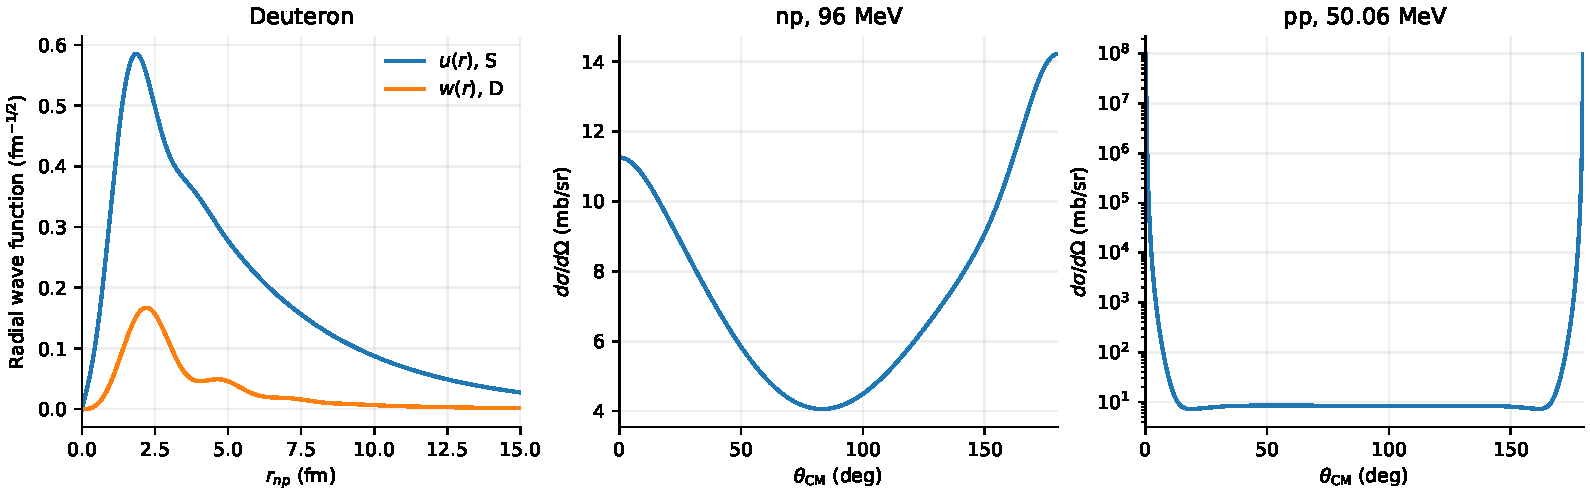
\includegraphics[width=\linewidth,height=.72\textheight,keepaspectratio]{说明书素材/example_outputs.pdf}\end{center}


图1。左图为氘核坐标 S/D 径向波函数，横轴是两核子的相对距离。中图为96 MeV np角分布。右图为50.06 MeV pp角分布，采用对数纵轴以显示库仑端点增长。三图展示本章范例运行产生的 Fortran 计算结果；与实验的比较见第9章。

若要改算另一个 np 能量，先完成本次归档，再复制输入为新文件，例如：


\begin{Verbatim}[samepage=true,breaklines=true,breakanywhere=true,fontsize=\small,frame=leftline,framesep=3mm,rulecolor=\color{bluegray}]
cp input_np.nml input_np_trial.nml
vi input_np_trial.nml
./run.sh input_np_trial.nml
\end{Verbatim}
在编辑器中修改 {\ttfamily\small energy\_\allowbreak{}lab\_\allowbreak{}MeV} 并保存，运行后从 {\ttfamily\small np\_\allowbreak{}summary.\allowbreak{}txt} 核对程序实际使用的能量。同样的方法可改变 pp 能量或数值参数。对照本章结果时，先保持原输入，确认基线复现后再改变参数。

\Needspace{6\baselineskip}\subsection*{7.7 后台运行、清理与重新编译}\addcontentsline{toc}{subsection}{7.7 后台运行、清理与重新编译}
日常任务可直接自动归档，或在当前机器后台执行：


\begin{Verbatim}[samepage=true,breaklines=true,breakanywhere=true,fontsize=\small,frame=leftline,framesep=3mm,rulecolor=\color{bluegray}]
./submit.sh input_np.nml
\end{Verbatim}
终端返回后台进程号。任务运行期间，可读取根目录 {\ttfamily\small run.\allowbreak{}log}；成功归档后，日志与结果一同位于按结束时间命名的目录。{\ttfamily\small submit.\allowbreak{}sh} 使用 nohup 启动当前机器上的后台任务，通常可在关闭终端后继续运行。关闭该计算机或终止进程会中断计算；当前两体任务没有断点续算功能，重启后需从头计算。使用 Slurm/PBS 的服务器应通过其队列系统提交任务，在队列脚本中进入程序根目录并调用 {\ttfamily\small .\allowbreak{}/\allowbreak{}run.\allowbreak{}sh 输入文件}。

同一根目录使用固定结果文件名，任务依次运行；并行计算使用各自独立的工作副本。清理和重新编译应在该工作副本的任务结束后进行。


\begin{Verbatim}[samepage=true,breaklines=true,breakanywhere=true,fontsize=\small,frame=leftline,framesep=3mm,rulecolor=\color{bluegray}]
./remove.sh
./remake.sh
make
\end{Verbatim}
第一条会删除根目录已知的过程/结果文件，\textbf{包括尚未归档的结果}；需要保留时先归档或移走。第二条清理 {\ttfamily\small app/\allowbreak{}} 的编译产物，第三条从源码重新构建。这两条清理脚本均保留已归档的 {\ttfamily\small output/\allowbreak{}}、日常输入和源码。日常任务成功归档后可直接继续运行；需要丢弃根目录运行文件时使用 {\ttfamily\small remove.\allowbreak{}sh}，需要重新构建时使用 {\ttfamily\small remake.\allowbreak{}sh} 和 {\ttfamily\small make}。

迁移服务器后，建议先执行 {\ttfamily\small .\allowbreak{}/\allowbreak{}remake.\allowbreak{}sh} 再 {\ttfamily\small make}。默认配置使用随包数学库。选择已安装的系统库时，可用 {\ttfamily\small make LINALG=\allowbreak{}system LIBS=\allowbreak{}"-llapack -lblas"}；切换前应清理编译产物，重建后重新验证。编译选项应保持已核验的浮点运算和数值接口约定，避免使用会改变这些约定的 {\ttfamily\small -ffast-math}、{\ttfamily\small -fdefault-real-8} 或 {\ttfamily\small -fdefault-integer-8}。

\Needspace{6\baselineskip}\subsection*{7.8 常见问题的处理}\addcontentsline{toc}{subsection}{7.8 常见问题的处理}

{\small\setlength{\tabcolsep}{3pt}\renewcommand{\arraystretch}{1.28}
\begin{longtable}{@{}>{\raggedright\arraybackslash}p{0.2784\linewidth}>{\raggedright\arraybackslash}p{0.3264\linewidth}>{\raggedright\arraybackslash}p{0.3552\linewidth}@{}}\toprule
\textbf{提示或现象} & \textbf{含义} & \textbf{处理方式}\\\midrule
\endfirsthead
\textbf{提示或现象} & \textbf{含义} & \textbf{处理方式}\\\midrule
\endhead
{\ttfamily\small Compile first: make} & 找不到可执行程序 & 在根目录执行make\\
{\ttfamily\small Existing runtime file} & 上次结果还在根目录 & 成功任务先归档；失败任务先查日志并保存现场\\
{\ttfamily\small A run lock exists} & 有活动任务或异常退出留下锁 & 先查任务是否仍运行，确认已停止才处理遗留空锁\\
{\ttfamily\small Invalid calculation\_\allowbreak{}input} & 输入格式或字段错误 & 检查引号、逗号、参数名及末尾 {\ttfamily\small /\allowbreak{}}\\
pp角度不合法 & 输入碰到0°或180° & 改为严格位于两端之间的角域\\
在壳q超出积分上限 & 当前积分区间不含奇点 & 核对能量与上限，也检查模型适用范围\\
在壳q与节点重合 & 主值离散分母为零 & 保持物理能量，换一个 {\ttfamily\small n\_\allowbreak{}grid} 并做稳定性检查\\
程序失败或被中断 & 本次没有成功归档 & 阅读根目录run.log，保留现场，处理原因后重新运行\\
\bottomrule\end{longtable}}
不同编译器和数学库可能在浮点末位有差别。复现以物理量和残差是否满足给定容差为判据。

\clearpage\section*{第8章 数值收敛与程序验证}\addcontentsline{toc}{section}{第8章 数值收敛与程序验证}
\Needspace{6\baselineskip}\subsection*{8.1 残差、收敛和实验一致性}\addcontentsline{toc}{subsection}{8.1 残差、收敛和实验一致性}
程序验证与精度评价分为几个层次。方程残差衡量离散矩阵的求解精度；改变网格、积分上限和分波截断，检验离散近似的收敛性；归一化与截面恒等式检查计算链的内部一致性。在这些检查的基础上，与实验比较可评价当前物理模型的描述能力。


{\small\setlength{\tabcolsep}{3pt}\renewcommand{\arraystretch}{1.28}
\begin{longtable}{@{}>{\raggedright\arraybackslash}p{0.2784\linewidth}>{\raggedright\arraybackslash}p{0.3264\linewidth}>{\raggedright\arraybackslash}p{0.3552\linewidth}@{}}\toprule
\textbf{检查层次} & \textbf{检查方法} & \textbf{检查范围与后续工作}\\\midrule
\endfirsthead
\textbf{检查层次} & \textbf{检查方法} & \textbf{检查范围与后续工作}\\\midrule
\endhead
离散方程的求解 & 本征/线性残差、互易性 & 核验当前矩阵解，再检查连续积分的离散误差\\
数值参数的收敛 & 独立改变节点、上限、分波等 & 评估数值截断误差，并单独说明模型采用的物理近似\\
概率与单位的一致性 & 归一化、幺正性、独立截面计算 & 核验计算链的内部一致性，再逐角度比较实验\\
模型与实验的比较 & 匹配定义后比较实验 & 评估描述能力，并结合数值、模型及实验因素分析差异\\
\bottomrule\end{longtable}}
\Needspace{6\baselineskip}\subsection*{8.2 氘核的逐项检查}\addcontentsline{toc}{subsection}{8.2 氘核的逐项检查}
在其他条件相同时，可把 {\ttfamily\small n\_\allowbreak{}grid} 依次设为 100、160、192、240，记录结合能、D 态概率和半径的变化。随后固定节点数，检查允许范围内的 {\ttfamily\small pmax\_\allowbreak{}MeV}，例如 800、900、1000。每次改变一个参数，其余设置保持一致，以识别各项数值近似的影响。

坐标观测量还要检查相对距离上限和步长。输入规定的是区间数：\(\Delta r=r_{\max}/N_r\)。比较步长时，保持 \(r_{\max}\) 不变；比较上限时，尽量保持 \(\Delta r\) 不变。尾拟合窗口位于 20—25 fm，输出 {\ttfamily\small tail\_\allowbreak{}fit\_\allowbreak{}available} 为 false 时，相关零值是占位值。

现有专项核查已包括动量/坐标归一化、Gaussian 波函数解析检验，以及独立动量微分公式求半径。N=192、相对距离上限60 fm、步长0.01 fm时，坐标归一化偏离1约 \(1.4\times10^{-12}\)；两种半径计算差约 \(3.5\times10^{-10}\) fm。这些数值给出了该范例坐标变换的数值精度；电磁量的物理精度还取决于第3.5节所述的算符近似及修正。

\Needspace{6\baselineskip}\subsection*{8.3 np 的网格与分波检查}\addcontentsline{toc}{subsection}{8.3 np 的网格与分波检查}
首先固定能量和 {\ttfamily\small jmax}，改变 {\ttfamily\small n\_\allowbreak{}grid}，比较完整角分布及在壳矩阵。其次固定网格，逐步提高 {\ttfamily\small jmax}，查看 {\ttfamily\small np\_\allowbreak{}j\_\allowbreak{}convergence.\allowbreak{}csv}。总截面与逐角度的微分截面应同时比较，特别关注前后角和截面极小处的干涉变化。

{\ttfamily\small n\_\allowbreak{}angles} 控制输出角度的采样密度，从181增加到721可得到更细的曲线。第4章主值方程的动量积分精度由 {\ttfamily\small n\_\allowbreak{}grid} 等参数控制。程序内部另行在完整角域上求积，用于积分截面检查；该角积分与用户指定的输出角度窗口分别设置。

研究计算应明确设置 {\ttfamily\small jmax}，并通过逐步增加该值确定所需分波范围。已有199.9 MeV检查中，J≤8与J≤32的180°截面相差约6\%。因此，默认的 {\ttfamily\small jmax=\allowbreak{}8} 可作为起始设置，高角动量在特定角度的贡献需要结合完整角分布检验。

np 模型只含弹性通道，因而理论上 \(S^\dagger S=I\)。从 S 矩阵求积分截面、从角分布积分、从前向振幅用光学定理求截面，三条路径应相互一致。这项闭合检查针对给定分波范围内的计算一致性；分波收敛则通过扩大该范围、比较观测量的变化来检验。

\Needspace{6\baselineskip}\subsection*{8.4 pp 的额外检查}\addcontentsline{toc}{subsection}{8.4 pp 的额外检查}
pp 除动量和角动量参数外，还有库仑匹配半径 {\ttfamily\small coulomb\_\allowbreak{}radius\_\allowbreak{}fm} 与径向求积点 {\ttfamily\small n\_\allowbreak{}coulomb\_\allowbreak{}points}。检查时分别改变它们，关注核—库仑干涉区域以及前角。输出应满足未极化相同质子角分布的 \(\theta\leftrightarrow180^\circ-\theta\) 对称性。

现有检验包括纯库仑极限、关闭库仑后的桥接、特殊函数、交换反对称化和干涉相位。完整九能量计算中，匹配后的幺正性误差约在 \(10^{-15}\) 量级。另在有限动量上限的纯库仑检验中，核背景矩阵 \(S_C\) 偏离单位阵可达约 \(1.21\times10^{-5}\)。前者检验匹配后矩阵的幺正性，后者反映纯库仑极限下的计算偏差；其中由动量上限引起的截尾误差，需要通过上限敏感性检查识别。

主程序将 {\ttfamily\small pmax\_\allowbreak{}MeV} 的允许范围设为大于0且不超过1000，这是程序当前允许的输入范围。已有开发检查可用于识别截尾效应；研究中若需系统提高上限，应先验证更高动量接口和库仑数值算法，再扩展允许的输入范围。模型的物理适用范围另按第2.6节评价。

pp 的全角库仑截面发散，积分截面检查应选用严格位于端点之间的有限角区间，并明确记录积分范围及相同粒子计数约定。

\Needspace{6\baselineskip}\subsection*{8.5 运行现有测试}\addcontentsline{toc}{subsection}{8.5 运行现有测试}
在没有正在运行的任务时，在根目录顺序执行：


\begin{Verbatim}[samepage=true,breaklines=true,breakanywhere=true,fontsize=\small,frame=leftline,framesep=3mm,rulecolor=\color{bluegray}]
make verify-sources
make check
\end{Verbatim}
两个目标均先按第7.1节准备并校验 COUL90外部依赖。第一条随后检查 {\ttfamily\small app/\allowbreak{}provenance/\allowbreak{}em500\_\allowbreak{}sources.\allowbreak{}sha256} 所记原核力、随包数学依赖、COUL90源码与冻结参考的哈希。第二条编译运行 {\ttfamily\small app/\allowbreak{}tests/\allowbreak{}} 中的六个 Fortran 验证程序，所需冻结参考保存在 {\ttfamily\small app/\allowbreak{}tests/\allowbreak{}reference/\allowbreak{}}。完成外部依赖准备后，测试可离线执行。测试与主程序编译共用模块文件，因此同一根目录中的 {\ttfamily\small make check} 和重新编译应依次执行。


{\small\setlength{\tabcolsep}{3pt}\renewcommand{\arraystretch}{1.28}
\begin{longtable}{@{}>{\raggedright\arraybackslash}p{0.3705\linewidth}>{\raggedright\arraybackslash}p{0.6045\linewidth}@{}}\toprule
\textbf{验证源码（均在 {\ttfamily\small app/\allowbreak{}tests/\allowbreak{}}）} & \textbf{检查对象}\\\midrule
\endfirsthead
\textbf{验证源码（均在 {\ttfamily\small app/\allowbreak{}tests/\allowbreak{}}）} & \textbf{检查对象}\\\midrule
\endhead
{\ttfamily\small check\_\allowbreak{}reference.\allowbreak{}f90} & 核力矩阵元、氘核能量及有符号S/D波函数与冻结参考的回归\\
{\ttfamily\small check\_\allowbreak{}deuteron\_\allowbreak{}observables.\allowbreak{}f90} & 坐标变换、密度及观测量的解析模型检验\\
{\ttfamily\small check\_\allowbreak{}np\_\allowbreak{}solver.\allowbreak{}f90} & 有限积分上限下的解析势模型、主值方程和耦合通道\\
{\ttfamily\small check\_\allowbreak{}np\_\allowbreak{}observables.\allowbreak{}f90} & 自旋与角动量重构、相位、角积分和光学定理\\
{\ttfamily\small check\_\allowbreak{}pp\_\allowbreak{}solver.\allowbreak{}f90} & 库仑特殊函数、匹配、关闭库仑后的桥接与求解\\
{\ttfamily\small check\_\allowbreak{}pp\_\allowbreak{}observables.\allowbreak{}f90} & 纯库仑极限、相同粒子交换、干涉相位与非法输入\\
\bottomrule\end{longtable}}
冻结参考生成于语言迁移前，作为固定的回归基准保留；运行当前求解器时应保持这些文件不变。文件含义和来源见 {\ttfamily\small app/\allowbreak{}tests/\allowbreak{}reference/\allowbreak{}README.\allowbreak{}md}、{\ttfamily\small reference\_\allowbreak{}manifest.\allowbreak{}json}，容差与判据以各测试源码为准。氘核回归的主要容差为能量 \(10^{-8}\) MeV、S/D概率 \(10^{-9}\)、动能/势能 \(10^{-7}\) MeV、有符号S/D联合加权距离 \(10^{-8}\)。这些容差为不同机器产生的浮点末位差异留有余量。

历史语言迁移另有新旧散射实现的完整角分布对照和独立算法对照，与随包六项测试共同构成程序验证记录。{\ttfamily\small make check} 复现上表列出的六项检查，历史迁移对照的摘要保存在 {\ttfamily\small app/\allowbreak{}provenance/\allowbreak{}np\_\allowbreak{}migration\_\allowbreak{}reference.\allowbreak{}json}。实验比较的数值稳定性与现有偏差见三个 {\ttfamily\small output/\allowbreak{}*\_\allowbreak{}com\_\allowbreak{}exp\_\allowbreak{}cal/\allowbreak{}} 目录及本书第9章。

现有程序验证覆盖原核力矩阵元与历史配置的一致性、不同求解实现的对照、解析简化模型及物理恒等式。共享同一核力源码的求解器对照，主要核验外围求解和观测量实现；核力源码自身的独立核验还需要外部参考。后续应单独记录与作者结果的完整对照，并统一 EM500 配置、电磁处理和各项约定。

\clearpage\section*{第9章 实验比较与结果解释}\addcontentsline{toc}{section}{第9章 实验比较与结果解释}
\Needspace{6\baselineskip}\subsection*{9.1 实验定义与比较条件}\addcontentsline{toc}{subsection}{9.1 实验定义与比较条件}
实验比较首先需要统一入射能量、角度参考系、出射粒子和计数方式。本程序的 {\ttfamily\small energy\_\allowbreak{}lab\_\allowbreak{}MeV} 表示入射粒子轰击静止靶核子的实验室动能，输出角度采用质心系。np 角分布对应出射中子；使用出射质子的数据时，需按实验定义转换角度。pp 数据的比较还需采用一致的相同粒子计数约定。

微分截面 CSV 采用 mb/sr，振幅采用 fm，换算为 \(1\ {\rm fm}^2=10\ {\rm mb}\)。实验数据的单位和归一化以原始论文及数据记录为依据，所做换算应保留出处。出现量级异常时，先核对这些定义。共同归一化误差会使同组数据点相关，统计比较应将这种相关性计入 \(\chi^2\)。

当前九能量图通过读取或插值理论曲线，得到实验角度处的计算值。比较采用名义入射能量，束流能谱和角接受度的卷积尚待处理。对于较宽的能量分箱，实验结果代表箱内平均；进一步的精密比较需要按实验能量分布和接受度对理论结果取平均。

\Needspace{6\baselineskip}\subsection*{9.2 氘核观测量比较}\addcontentsline{toc}{subsection}{9.2 氘核观测量比较}
下表列出当前固定模型的代表结果，备注注明了所用算符近似。完整实验来源、不确定度和详细表保存在 {\ttfamily\small output/\allowbreak{}d\_\allowbreak{}com\_\allowbreak{}exp\_\allowbreak{}cal/\allowbreak{}}。


{\small\setlength{\tabcolsep}{3pt}\renewcommand{\arraystretch}{1.28}
\begin{longtable}{@{}>{\raggedright\arraybackslash}p{0.235\linewidth}>{\raggedright\arraybackslash}p{0.235\linewidth}>{\raggedright\arraybackslash}p{0.235\linewidth}>{\raggedright\arraybackslash}p{0.235\linewidth}@{}}\toprule
\textbf{观测量} & \textbf{当前计算} & \textbf{实验/分析值} & \textbf{备注}\\\midrule
\endfirsthead
\textbf{观测量} & \textbf{当前计算} & \textbf{实验/分析值} & \textbf{备注}\\\midrule
\endhead
结合能（MeV） & 2.22457528 & 2.2245662(4) & 核力曾按历史结合能定参\\
电荷半径（fm） & 2.126774 & 2.12778(27) & 有限核子尺寸+DF估计\\
电四极矩（fm²） & 0.274951 & 0.285699 & 单体脉冲近似\\
磁矩（核磁子） & 0.854087 & 0.8574382335 & 单体脉冲近似\\
渐近 S 波归一常数（\(\mathrm{fm}^{-1/2}\)） & 0.884303 & 0.8845(8) & 散射分析提取\\
渐近 D/S 比 & 0.0255807 & 0.0256(4) & 反应分析提取\\
\bottomrule\end{longtable}}
计算结合能与现代质量表相差约9 eV。解释这一差别时，需要核对核力的历史拟合目标，并将其与固定模型下的动量网格误差分别考察。四极矩和磁矩同时依赖波函数与电磁算符，后续精度改进还包括完整的二体电磁贡献。D态概率约4.514\%，适合作为同一核力表示下的数值诊断量；它依赖所采用的表示，实验可约束的是相应的物理观测量。

\Needspace{6\baselineskip}\subsection*{9.3 np 与 pp 的九能量研究材料}\addcontentsline{toc}{subsection}{9.3 np 与 pp 的九能量研究材料}

{\small\setlength{\tabcolsep}{3pt}\renewcommand{\arraystretch}{1.28}
\begin{longtable}{@{}>{\raggedright\arraybackslash}p{0.2784\linewidth}>{\raggedright\arraybackslash}p{0.3264\linewidth}>{\raggedright\arraybackslash}p{0.3552\linewidth}@{}}\toprule
\textbf{体系} & \textbf{实验室能量（MeV）} & \textbf{资料目录}\\\midrule
\endfirsthead
\textbf{体系} & \textbf{实验室能量（MeV）} & \textbf{资料目录}\\\midrule
\endhead
np & 3.1、10.04、25.8、50、96、137、150、200、300.2 & {\ttfamily\small output/\allowbreak{}np\_\allowbreak{}com\_\allowbreak{}exp\_\allowbreak{}cal/\allowbreak{}}\\
pp & 3.037、9.69、14.16、50.06、98、142、239.9、270.8、286.7 & {\ttfamily\small output/\allowbreak{}pp\_\allowbreak{}com\_\allowbreak{}exp\_\allowbreak{}cal/\allowbreak{}}\\
\bottomrule\end{longtable}}
每个目录包含实验数据及来源、Fortran 输入与运行结果、比较数据和画图脚本。各能量的数据覆盖范围不同，例如部分低能 np 数据只有少数独立角度。计算曲线给出模型在完整角域的结果，实验检验范围则由实际测量的角度确定。

np 的300.2 MeV原相对角分布按论文给出的归一化量转成绝对值，并保留共同归一化误差信息。该能量的计算在约80°处偏高、后角偏低，表明差异涉及角分布形状，需要随角度分析。

pp 在部分能区的形状和量级接近实验。现有98 MeV数据在前角10.2°处仍有明显偏差：计算约6.20 mb/sr，实验约12.4 mb/sr。这一偏差的来源尚待确定，后续核查应涵盖完整电磁方案、采用同一核力的外部计算以及实验处理。现有数值检验为求解过程提供了依据，实验符合程度还需按能量和角度分别评价。


\clearpage
\subsubsection*{np：九个入射能量的实验与计算}

\begin{center}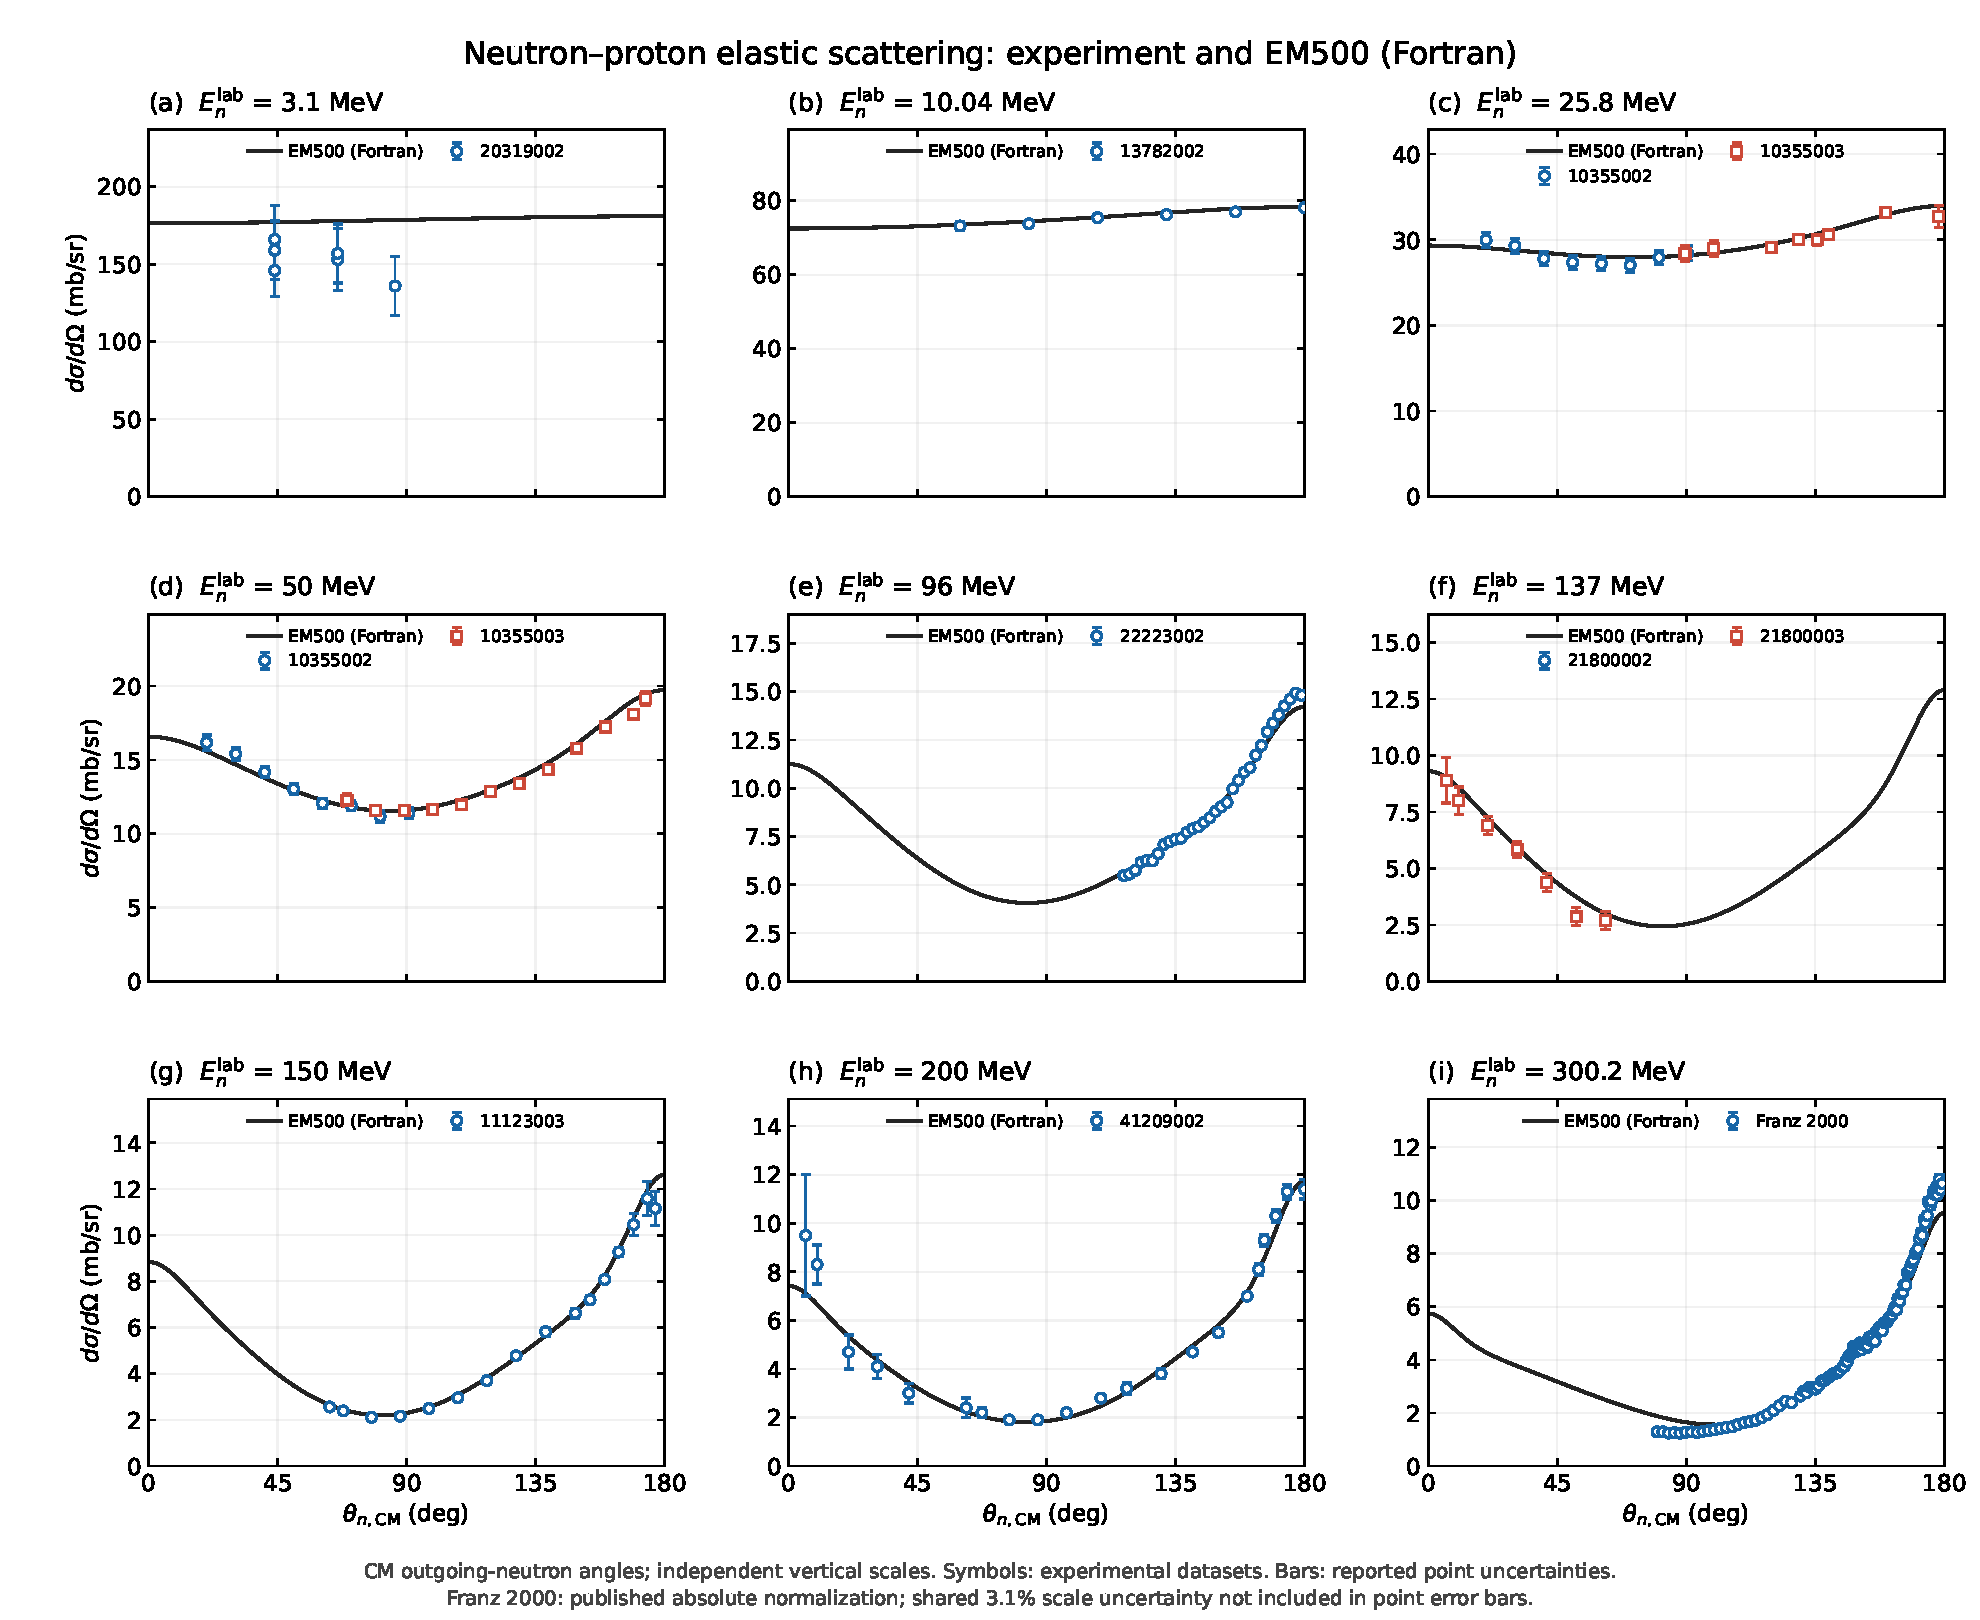
\includegraphics[width=\linewidth,height=.72\textheight,keepaspectratio]{../output/np_com_exp_cal/np_exp_cal_angular_3x3.pdf}\end{center}


图2。np 弹性散射九能量角分布。各子图标题给出入射中子的实验室动能，横轴为质心系（CM）出射中子角度，纵轴为微分截面，单位 mb/sr；各子图采用独立的线性纵轴范围。曲线来自固定 EM500 核力的 Fortran 求解，理论归一化由模型确定；数据点及误差棒来自实验。最后一个子图采用 \textbf{300.2 MeV} 数据与计算。前八个能量的数据来自 EXFOR；300.2 MeV来自 Franz 等的20 MeV能量分箱数据，按论文归一化量转成绝对截面，其3.1\%共同归一化不确定度作为整组数据的相关误差单独保留。图中误差棒采用原记录给出的逐点误差信息，理论采用名义能量，实验能谱和角接受度的卷积尚待处理。实验检验限于数据点覆盖的角域，高能偏差的讨论见本节前文。数据来源、输入和运行记录见 {\ttfamily\small output/\allowbreak{}np\_\allowbreak{}com\_\allowbreak{}exp\_\allowbreak{}cal/\allowbreak{}}。


\clearpage
\subsubsection*{pp：九个入射能量的实验与计算}

\begin{center}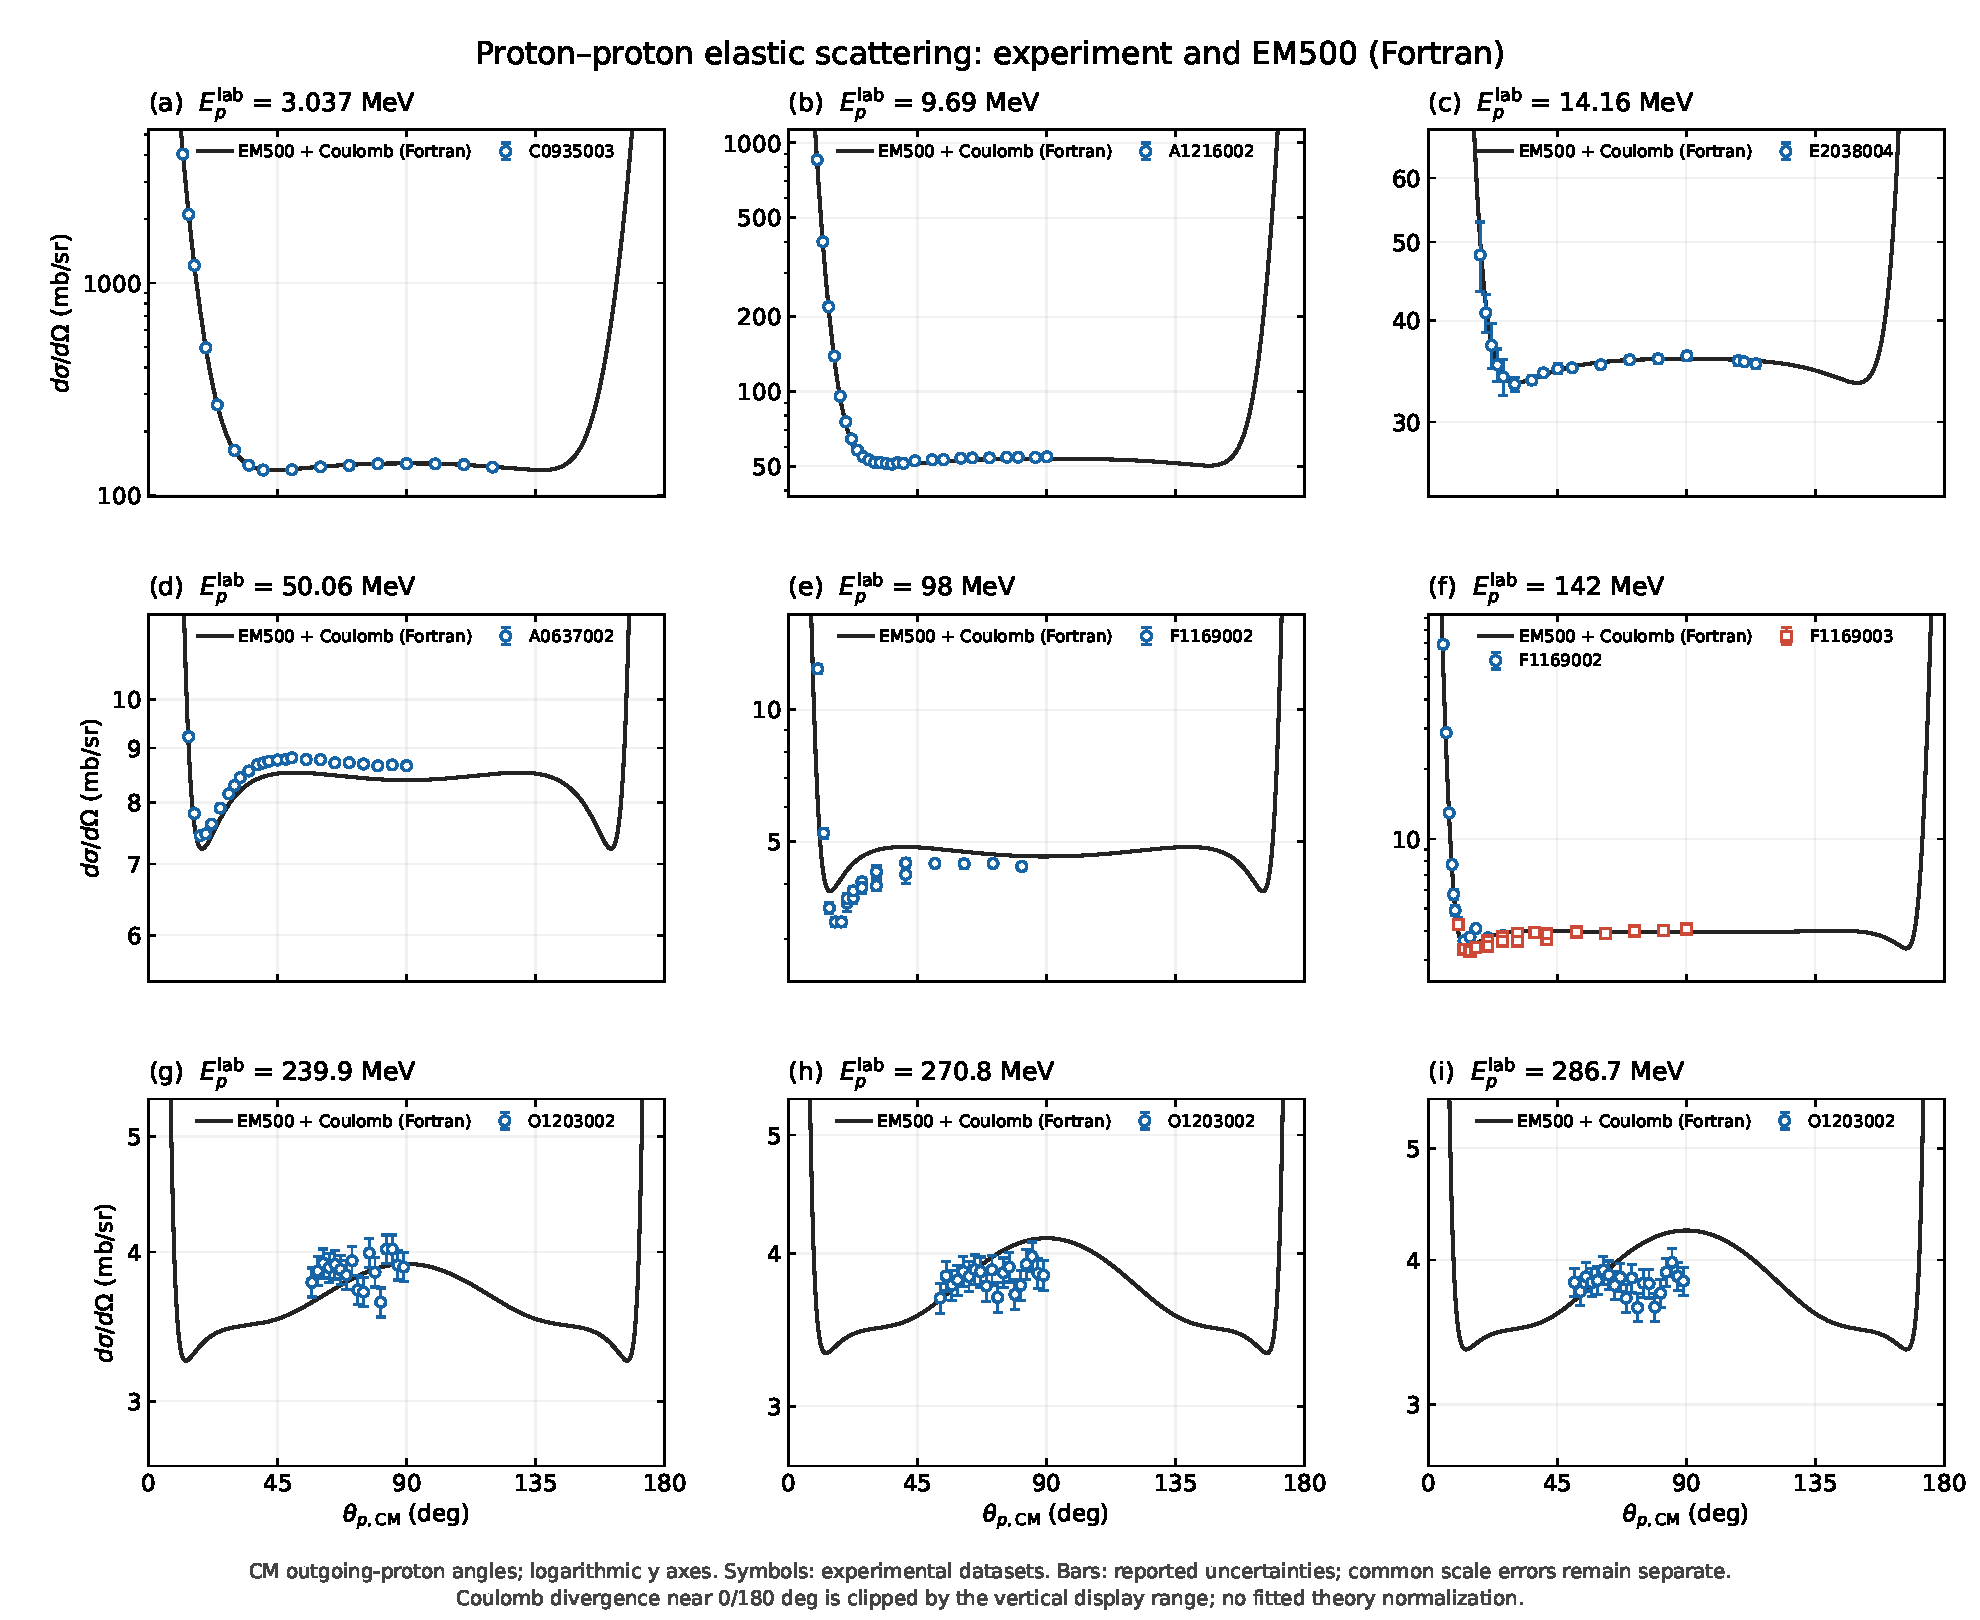
\includegraphics[width=\linewidth,height=.72\textheight,keepaspectratio]{../output/pp_com_exp_cal/pp_exp_cal_angular_3x3.pdf}\end{center}


图3。pp 弹性散射九能量角分布。各子图标题给出入射质子的实验室动能，横轴为质心系（CM）角度，纵轴为微分截面，单位 mb/sr；\textbf{纵轴采用对数坐标}，各子图范围独立。曲线来自含当前库仑方案与相同粒子交换处理的 Fortran 求解，理论归一化由模型确定。EXFOR实验点按原记录的角度和数值绘制，保留实际测量的角度覆盖范围。前后向库仑尖峰可能超出纵轴显示范围；积分计算的角域应依据所需观测量单独规定。多组数据另有共同归一化不确定度，统计分析需结合误差棒信息及这种相关误差。98 MeV前角的明显偏差见本节前文，相关来源仍需进一步核查。数据来源、输入和运行记录见 {\ttfamily\small output/\allowbreak{}pp\_\allowbreak{}com\_\allowbreak{}exp\_\allowbreak{}cal/\allowbreak{}}。


\clearpage
\Needspace{6\baselineskip}\subsection*{9.4 差异来源的逐层分析}\addcontentsline{toc}{subsection}{9.4 差异来源的逐层分析}
差异分析可按以下顺序进行：首先统一实验与计算的物理定义，再完成第8章的数值参数变化检查；随后对照解析模型和独立实现，最后考察固定核力的有限阶误差、电磁算符近似及高能开放通道。每一层检查都对应明确的比较对象，便于量化改进的效果。

增加网格后结果趋于稳定，是该数值参数收敛的证据。保存相应结果后，可继续考察其他误差来源。更换核力、调节器或算符时，应建立新的模型记录，与原结果并列保存，使模型变化、数值变化及实验符合程度都可追溯。

\clearpage\section*{附录A 符号与单位速查}\addcontentsline{toc}{section}{附录A 符号与单位速查}

{\small\setlength{\tabcolsep}{3pt}\renewcommand{\arraystretch}{1.28}
\begin{longtable}{@{}>{\raggedright\arraybackslash}p{0.2784\linewidth}>{\raggedright\arraybackslash}p{0.3264\linewidth}>{\raggedright\arraybackslash}p{0.3552\linewidth}@{}}\toprule
\textbf{对象} & \textbf{本程序约定} & \textbf{使用说明}\\\midrule
\endfirsthead
\textbf{对象} & \textbf{本程序约定} & \textbf{使用说明}\\\midrule
\endhead
动量 \(p,q\) & MeV/c，计算中 \(c=1\) & 通过所选运动学关系与入射能量换算\\
能量 \(E,B\) & MeV；束缚态 \(E=-B\) & 束缚态本征能量为负，结合能为正\\
质量参数 \(m\) & np 为两倍约化质量；pp 为质子质量 & 质量参数已包含约化质量中的相应因子，按本书相对动能公式使用\\
分波势 \(V\)、在壳 \(K,T\) & MeV⁻²，测度 \(dp\,p^2\) & 积分方程采用上述测度；相应归一化中已处理 \(2/\pi\)\\
动量波函数 \(\psi_L\) & \(\mathrm{MeV}^{-3/2}\) & 按定义分别读取原函数与 \(p\psi_L\)\\
坐标约化函数 \(u,w\) & \(\mathrm{fm}^{-1/2}\)，\(\int dr(u^2+w^2)=1\) & \(u^2+w^2\) 是相对距离的径向概率密度，体密度需作相应几何换算\\
\(r,R\)（氘核后处理） & 核子间距、距等质量质心距离；\(R=r/2\) & 点核子空间密度以距质心距离R为自变量\\
\(R\)（pp匹配） & 库仑匹配半径 & 在pp外区匹配公式中表示内外区的连接半径\\
散射振幅 \(f\) & fm & 振幅平方按面积单位换算为mb\\
角分布 & mb/sr、质心系角度 & 与实验比较时统一角度参考系及截面单位\\
\(S\) 与 \(\mathsf S\) & 总自旋与散射矩阵，依上下文区分 & 前者标记自旋通道，后者描述散射初末态关系\\
\(T_{\rm iso}\) 与 \(T\) & 同位旋与散射算符 & 同位旋标签用于确定允许通道，计数按相应自旋平均和通道求和公式执行\\
\bottomrule\end{longtable}}
\clearpage\section*{附录B EM500接口与来源}\addcontentsline{toc}{section}{附录B EM500接口与来源}
\Needspace{6\baselineskip}\subsection*{B.1 固定上游与原始分量}\addcontentsline{toc}{subsection}{B.1 固定上游与原始分量}
上游仓库为 \href{https://github.com/seanbsm/Tic-tac}{seanbsm/Tic-tac}，本包冻结提交：


\begin{Verbatim}[samepage=true,breaklines=true,breakanywhere=true,fontsize=\small,frame=leftline,framesep=3mm,rulecolor=\color{bluegray}]
30338ac0eaf968b6db2edfa8380410651a56267b
\end{Verbatim}
{\ttfamily\small app/\allowbreak{}provenance/\allowbreak{}upstream.\allowbreak{}json} 保存原始网址和哈希，{\ttfamily\small app/\allowbreak{}provenance/\allowbreak{}em500\_\allowbreak{}sources.\allowbreak{}sha256} 用于核验。上游许可随 {\ttfamily\small app/\allowbreak{}em500/\allowbreak{}} 保存。包内核力代码采用这一公开实现的固定副本。与其他 EM500 实现比对时，需要统一归一化、相位和电磁处理约定。

原始 {\ttfamily\small chp} 返回 {\ttfamily\small raw(6)}。本接口依据源码的实际执行定义，以 {\ttfamily\small pout} 为输出动量、{\ttfamily\small pin} 为输入动量。上游参数注释存在歧义，接口的调用顺序以这里记录的执行定义为准。


{\small\setlength{\tabcolsep}{3pt}\renewcommand{\arraystretch}{1.28}
\begin{longtable}{@{}>{\raggedright\arraybackslash}p{0.3705\linewidth}>{\raggedright\arraybackslash}p{0.6045\linewidth}@{}}\toprule
\textbf{类型} & \textbf{本接口使用的分量}\\\midrule
\endfirsthead
\textbf{类型} & \textbf{本接口使用的分量}\\\midrule
\endhead
自旋单态，非耦合 & {\ttfamily\small v(1,1)=\allowbreak{}raw(1)}\\
自旋三重态，非耦合 & {\ttfamily\small v(1,1)=\allowbreak{}raw(2)}\\
三重态 J=0，即 ³P₀ & {\ttfamily\small v(1,1)=\allowbreak{}raw(3)}，API仍用 {\ttfamily\small coupled=\allowbreak{}.\allowbreak{}true.\allowbreak{}}\\
三重态 J>0，耦合 & {\ttfamily\small v(1,1)=\allowbreak{}raw(4)}，{\ttfamily\small v(1,2)=\allowbreak{}raw(6)}，{\ttfamily\small v(2,1)=\allowbreak{}raw(5)}，{\ttfamily\small v(2,2)=\allowbreak{}raw(3)}\\
\bottomrule\end{longtable}}
耦合通道顺序为 \(L=J-1,J+1\)。接口核验采用 \(p'\ne p\) 的点，以分别检验输入和输出动量的映射。pp 设 \(T_{\rm iso}=1,t_z=-1\)，np 使用 \(t_z=0\)。

\Needspace{6\baselineskip}\subsection*{B.2 参数与相位的复现要求}\addcontentsline{toc}{subsection}{B.2 参数与相位的复现要求}
35个输入值以 {\ttfamily\small app/\allowbreak{}em500\_\allowbreak{}parameters.\allowbreak{}f90} 和 {\ttfamily\small app/\allowbreak{}provenance/\allowbreak{}em500.\allowbreak{}json} 为准。本接口数组下标从1开始，上游形参数组下标从0开始。Fortran按数组元素顺序传递参数，因此本接口第1项直接对应上游第0项，其余各项依次对应。

例如当前配置 \(g_A=1.29\)，\((c_1,c_2,c_3,c_4)=(-0.81,2.80,-3.20,5.40)\) GeV⁻¹。接触参数经上游入口的单位换算后，才用于MeV制势核的装配。完整复现还需保留调节器、共同归一因子、选定图项和相位约定，它们共同组成模型定义。

原核力采用 {\ttfamily\small radial\_\allowbreak{}rephased} 基。氘核 S/D 波函数和坐标变换遵守这一约定；散射角展开则通过 \(U_{LL'}=i^L\delta_{LL'}\) 转到普通动量基。相位变换应同时作用于势、波函数和观测算符，以保持物理结果一致。

\Needspace{6\baselineskip}\subsection*{B.3 外部依赖与来源记录}\addcontentsline{toc}{subsection}{B.3 外部依赖与来源记录}
EM500与 LAPACK/BLAS 的固定源码及相应许可继续随包保存。COUL90采用“来源记录、固定哈希、用户端获取”的分发方式：{\ttfamily\small app/\allowbreak{}coulomb/\allowbreak{}UPSTREAM.\allowbreak{}json} 记录原站地址和文件校验值，{\ttfamily\small fetch\_\allowbreak{}external.\allowbreak{}sh} 负责获取或导入指定文件并校验。取得的 {\ttfamily\small app/\allowbreak{}coulomb/\allowbreak{}coul90.\allowbreak{}f} 作为本地构建依赖使用。联网获取和离线导入使用同一文件与相同校验标准，具体操作见第7.1节。

\clearpage\section*{附录C 输入输出速查}\addcontentsline{toc}{section}{附录C 输入输出速查}
\Needspace{6\baselineskip}\subsection*{C.1 输入参数}\addcontentsline{toc}{subsection}{C.1 输入参数}
所有参数都写在 {\ttfamily\small \&calculation\_\allowbreak{}input .\allowbreak{}.\allowbreak{}.\allowbreak{} /\allowbreak{}} 中。下表列出代码默认值和允许范围，第7章范例则显式指定了所用数值参数。


{\small\setlength{\tabcolsep}{3pt}\renewcommand{\arraystretch}{1.28}
\begin{longtable}{@{}>{\raggedright\arraybackslash}p{0.2784\linewidth}>{\raggedright\arraybackslash}p{0.3264\linewidth}>{\raggedright\arraybackslash}p{0.3552\linewidth}@{}}\toprule
\textbf{参数} & \textbf{默认值} & \textbf{含义/要求}\\\midrule
\endfirsthead
\textbf{参数} & \textbf{默认值} & \textbf{含义/要求}\\\midrule
\endhead
{\ttfamily\small calculation} & {\ttfamily\small deuteron\_\allowbreak{}bound\_\allowbreak{}state} & 可选氘核、{\ttfamily\small np\_\allowbreak{}scattering}、{\ttfamily\small pp\_\allowbreak{}scattering}\\
{\ttfamily\small system} & {\ttfamily\small np} & pp任务设为 {\ttfamily\small pp}\\
{\ttfamily\small interaction} & {\ttfamily\small EM500} & 当前实现的固定核力模型\\
{\ttfamily\small n\_\allowbreak{}grid} & 100 & 每轨道通道动量节点，4—1000\\
{\ttfamily\small pmax\_\allowbreak{}MeV} & 1000 & 积分上限，大于0且不超过1000；散射要求大于q\\
{\ttfamily\small energy\_\allowbreak{}lab\_\allowbreak{}MeV} & −1 & 散射取正数；氘核省略\\
{\ttfamily\small kinematics} & {\ttfamily\small nonrelativistic} & 或 {\ttfamily\small relativistic}；pp含有效库仑参数区别\\
{\ttfamily\small jmax} & 8 & 散射总J截断，0—39；正式范例显式为32\\
{\ttfamily\small theta\_\allowbreak{}min\_\allowbreak{}deg} & 0 & 质心角下限；pp取大于0的值\\
{\ttfamily\small theta\_\allowbreak{}max\_\allowbreak{}deg} & 180 & 质心角上限；pp取小于180的值\\
{\ttfamily\small n\_\allowbreak{}angles} & 181 & 输出角度点数，1—100001；为1时上下限相等\\
{\ttfamily\small write\_\allowbreak{}amplitudes} & {\ttfamily\small .\allowbreak{}true.\allowbreak{}} & 散射是否额外导出复振幅\\
{\ttfamily\small write\_\allowbreak{}matrices} & {\ttfamily\small .\allowbreak{}false.\allowbreak{}} & 氘核是否导出完整V/H矩阵\\
{\ttfamily\small write\_\allowbreak{}coordinate} & {\ttfamily\small .\allowbreak{}false.\allowbreak{}} & 氘核是否计算坐标波函数及观测量\\
{\ttfamily\small coordinate\_\allowbreak{}rmax\_\allowbreak{}fm} & 40 & 相对距离上限，启用时大于0且不超过1000\\
{\ttfamily\small coordinate\_\allowbreak{}n\_\allowbreak{}intervals} & 4000 & 坐标区间数，启用时为100—1000000内偶数\\
{\ttfamily\small coulomb\_\allowbreak{}radius\_\allowbreak{}fm} & 15 & pp匹配半径，1—100 fm；正式范例为16\\
{\ttfamily\small n\_\allowbreak{}coulomb\_\allowbreak{}points} & 192 & pp库仑径向积分点，8—4000\\
\bottomrule\end{longtable}}
\Needspace{6\baselineskip}\subsection*{C.2 观测量与输出文件}\addcontentsline{toc}{subsection}{C.2 观测量与输出文件}

{\small\setlength{\tabcolsep}{3pt}\renewcommand{\arraystretch}{1.28}
\begin{longtable}{@{}>{\raggedright\arraybackslash}p{0.3705\linewidth}>{\raggedright\arraybackslash}p{0.6045\linewidth}@{}}\toprule
\textbf{内容} & \textbf{文件/字段}\\\midrule
\endfirsthead
\textbf{内容} & \textbf{文件/字段}\\\midrule
\endhead
氘核结合能 & {\ttfamily\small deuteron\_\allowbreak{}summary.\allowbreak{}txt} 的 {\ttfamily\small binding\_\allowbreak{}MeV}\\
氘核波函数 & {\ttfamily\small deuteron\_\allowbreak{}wavefunction.\allowbreak{}csv}；启用坐标输出后另有 {\ttfamily\small deuteron\_\allowbreak{}coordinate\_\allowbreak{}wavefunction.\allowbreak{}csv}\\
半径、Q、磁矩、尾参数 & {\ttfamily\small deuteron\_\allowbreak{}observables.\allowbreak{}dat}\\
np角分布 & {\ttfamily\small np\_\allowbreak{}angular\_\allowbreak{}distribution.\allowbreak{}csv}\\
np积分截面与守恒检查 & {\ttfamily\small np\_\allowbreak{}summary.\allowbreak{}txt}\\
np分波矩阵与相移 & {\ttfamily\small np\_\allowbreak{}on\_\allowbreak{}shell.\allowbreak{}csv}、{\ttfamily\small np\_\allowbreak{}partial\_\allowbreak{}waves.\allowbreak{}csv}\\
pp角分布 & {\ttfamily\small pp\_\allowbreak{}angular\_\allowbreak{}distribution.\allowbreak{}csv}\\
pp库仑背景下核S矩阵 & {\ttfamily\small pp\_\allowbreak{}nuclear\_\allowbreak{}s.\allowbreak{}csv}\\
pp各通道量子数及诊断 & {\ttfamily\small pp\_\allowbreak{}partial\_\allowbreak{}waves.\allowbreak{}csv}（当前导出内容为量子数和数值诊断）\\
分波截断变化 & {\ttfamily\small np\_\allowbreak{}j\_\allowbreak{}convergence.\allowbreak{}csv}、{\ttfamily\small pp\_\allowbreak{}j\_\allowbreak{}convergence.\allowbreak{}csv}\\
已重建的复振幅 & {\ttfamily\small np\_\allowbreak{}spin\_\allowbreak{}amplitudes.\allowbreak{}csv}、{\ttfamily\small pp\_\allowbreak{}spin\_\allowbreak{}amplitudes.\allowbreak{}csv}\\
任务完成状态 & {\ttfamily\small run\_\allowbreak{}status.\allowbreak{}txt} 与 {\ttfamily\small run\_\allowbreak{}metadata.\allowbreak{}txt}\\
实际使用的输入 & 归档中的 {\ttfamily\small input.\allowbreak{}nml} 原始快照及 {\ttfamily\small *\_\allowbreak{}input.\allowbreak{}nml} 有效参数\\
本次程序版本和可执行文件哈希 & {\ttfamily\small run\_\allowbreak{}metadata.\allowbreak{}txt}\\
编译器与编译选项 & 相应 {\ttfamily\small *\_\allowbreak{}summary.\allowbreak{}txt} 中的记录\\
\bottomrule\end{longtable}}
\Needspace{6\baselineskip}\subsection*{C.3 脚本和版本文件}\addcontentsline{toc}{subsection}{C.3 脚本和版本文件}

{\small\setlength{\tabcolsep}{3pt}\renewcommand{\arraystretch}{1.28}
\begin{longtable}{@{}>{\raggedright\arraybackslash}p{0.3705\linewidth}>{\raggedright\arraybackslash}p{0.6045\linewidth}@{}}\toprule
\textbf{文件} & \textbf{功能}\\\midrule
\endfirsthead
\textbf{文件} & \textbf{功能}\\\midrule
\endhead
{\ttfamily\small fetch\_\allowbreak{}external.\allowbreak{}sh} & 获取并校验 COUL90；{\ttfamily\small --source 文件路径} 从已有本地文件导入\\
{\ttfamily\small run.\allowbreak{}sh} & 前台运行，默认成功后自动归档\\
{\ttfamily\small submit.\allowbreak{}sh} & 使用nohup在当前机器后台运行；Slurm/PBS队列另按调度系统要求提交\\
{\ttfamily\small archive\_\allowbreak{}run.\allowbreak{}sh} & 手动归档已完成结果，校验后清除根目录本次运行文件\\
{\ttfamily\small remove.\allowbreak{}sh} & 删除根目录已知运行结果/过程文件，包括尚未归档的结果\\
{\ttfamily\small remake.\allowbreak{}sh} & 清理app编译产物，保留源码，随后可重新make\\
{\ttfamily\small .\allowbreak{}gitignore} & 规定Git通常忽略的生成文件；文件备份另行安排\\
{\ttfamily\small SHA256SUMS} & 用于核查某一交付快照的文件一致性；版本沿革见版本历史记录\\
{\ttfamily\small VERSION} & 人工维护的软件版本号，在发布新版本时更新\\
{\ttfamily\small CHANGELOG.\allowbreak{}md} & 各版功能和目录变化的人工记录\\
\bottomrule\end{longtable}}
修改输入或源码后，文件哈希会相应变化。更新交付快照前，应核对这些变化是否与预期修改一致，再生成新的校验表并保存版本记录。每次正式结果至少保留输入、输出、代码版本/提交、源码或发布包以及运行日志。

\clearpage\section*{附录D 文档版本与依据}\addcontentsline{toc}{section}{附录D 文档版本与依据}
\Needspace{6\baselineskip}\subsection*{D.1 本文档对应的状态}\addcontentsline{toc}{subsection}{D.1 本文档对应的状态}
本文档 v0.3，修订日期为2026-09-30，对应公开代码包 {\ttfamily\small VERSION=\allowbreak{}0.\allowbreak{}5.\allowbreak{}2}。本版沿用v0.2的教学叙述，更新公开分发、外部依赖获取和使用说明。EM500参数、物理模型、求解算法、公式及既有计算数值保持不变。

代码包0.5.2的更新范围为公开发布的包装与分发方式。来源记录位于 {\ttfamily\small app/\allowbreak{}provenance/\allowbreak{}}，随包测试和冻结参考位于 {\ttfamily\small app/\allowbreak{}tests/\allowbreak{}}；COUL90按第7.1节准备，EM500与 LAPACK/BLAS 继续随包提供。版本历史统一见根目录 {\ttfamily\small CHANGELOG.\allowbreak{}md}。

历史来源文件 {\ttfamily\small app/\allowbreak{}provenance/\allowbreak{}em500.\allowbreak{}json} 中的 {\ttfamily\small pp\_\allowbreak{}coulomb\_\allowbreak{}included=\allowbreak{}false} 描述原核力接口；当前pp求解器另外加入库仑。该文件的迁移状态字段及 {\ttfamily\small package\_\allowbreak{}origin.\allowbreak{}json} 所记版本反映各自生成阶段的状态，相关模型与验证说明见本书第5、8章。当前包版本以根目录 {\ttfamily\small VERSION} 为准。

历史输出中的摘要标题可能保留pp扩展初始版本 v0.4.0。追溯具体计算时，以该次运行保存的版本、源码及可执行文件哈希为依据。共享计算入口为 {\ttfamily\small app/\allowbreak{}fewbody.\allowbreak{}x}。

第7.5节三个原始范例曾在独立目录从源码编译运行，本书沿用初版核验所得的数值记录。初版构建与运行记录保存在项目的 {\ttfamily\small runs/\allowbreak{}manual\_\allowbreak{}em500\_\allowbreak{}2026-09-29/\allowbreak{}}。这些测试检验了范例复现和指定回归项目；模型与实验的符合程度则按第8、9章的方法进一步评价。完整历史构建记录保存在发布包外的项目档案中。公开包保存所需输入、测试和PDF素材，编译与测试所需的 COUL90由第7.1节的获取步骤准备。

0.5.1精简包已另行通过从源码全新编译、{\ttfamily\small make verify-sources} 和 {\ttfamily\small make check}，并完成氘核、np、pp三个实际运行与自动归档；三次归档均通过文件哈希校验。测试使用包内的 {\ttfamily\small app/\allowbreak{}tests/\allowbreak{}} 与冻结参考，已有实验比较的数值数据和图沿用原记录。完整日志保存在发布包外的 {\ttfamily\small runs/\allowbreak{}github\_\allowbreak{}package\_\allowbreak{}cleanup\_\allowbreak{}2026-09-29/\allowbreak{}}。这些检查验证了整理后的构建、测试和运行流程，物理验证范围仍按第8、9章所列证据确定。

公开包保留三个 {\ttfamily\small output/\allowbreak{}*\_\allowbreak{}com\_\allowbreak{}exp\_\allowbreak{}cal/\allowbreak{}} 目录中的科学数据、计算结果和自制图；第三方论文全文、截图与网页快照通过来源链接查阅。各目录的 {\ttfamily\small SOURCE\_\allowbreak{}LINKS.\allowbreak{}md} 汇总相关来源，原始数据出处和处理说明继续随实验比较资料保存。上述分发调整保持既有数值结果和自制图不变。

\Needspace{6\baselineskip}\subsection*{D.2 在迁移后的代码包中重新生成PDF}\addcontentsline{toc}{subsection}{D.2 在迁移后的代码包中重新生成PDF}
{\ttfamily\small docs/\allowbreak{}build\_\allowbreak{}pdf.\allowbreak{}py} 负责文档排版，直接读取本目录的 Markdown、{\ttfamily\small 说明书素材/\allowbreak{}} 以及 {\ttfamily\small output/\allowbreak{}np\_\allowbreak{}com\_\allowbreak{}exp\_\allowbreak{}cal/\allowbreak{}}、{\ttfamily\small output/\allowbreak{}pp\_\allowbreak{}com\_\allowbreak{}exp\_\allowbreak{}cal/\allowbreak{}} 中已有的比较图片。图表所据的氘核数据保存在 {\ttfamily\small output/\allowbreak{}d\_\allowbreak{}com\_\allowbreak{}exp\_\allowbreak{}cal/\allowbreak{}}。保留这些目录即可在迁移后的代码包中生成PDF。排版直接使用已有图片，所需材料均在公开包内；COUL90准备、物理求解和实验数据提取属于独立工作步骤。

在代码包根目录执行：


\begin{Verbatim}[samepage=true,breaklines=true,breakanywhere=true,fontsize=\small,frame=leftline,framesep=3mm,rulecolor=\color{bluegray}]
python3 -m pip install -r docs/requirements-pdf.txt
python3 docs/build_pdf.py
\end{Verbatim}
环境还需 XeLaTeX、CTeX/Fandol中文字体、DejaVu字体及本书使用的常见TeX宏包。具体安装和独立使用TeX源文件的方法见 {\ttfamily\small docs/\allowbreak{}PDF生成说明.\allowbreak{}md}。脚本默认把编译中间文件放在系统临时目录，成功后更新本目录同名 {\ttfamily\small .\allowbreak{}tex} 与 {\ttfamily\small .\allowbreak{}pdf}；如需保存编译日志，可加 {\ttfamily\small --build-dir /\allowbreak{}自行选择的日志目录}。已有TeX源文件时，{\ttfamily\small python3 docs/\allowbreak{}build\_\allowbreak{}pdf.\allowbreak{}py --from-tex} 可跳过Markdown转换。

\Needspace{6\baselineskip}\subsection*{D.3 进一步阅读与原始资料}\addcontentsline{toc}{subsection}{D.3 进一步阅读与原始资料}
\begin{enumerate}[start=1]
\item Entem 与 Machleidt，2003，EM N³LO势原始论文：\href{https://doi.org/10.1103/PhysRevC.68.041001}{Phys. Rev. C 68, 041001}。


\item Machleidt 与 Entem，2011，手征核力与公式综述：\href{https://doi.org/10.1016/j.physrep.2011.02.001}{Phys. Rep. 503, 1–75}。


\item Vincent 与 Phatak，1974，动量空间库仑匹配方法：\href{https://doi.org/10.1103/PhysRevC.10.391}{Phys. Rev. C 10, 391}。


\item 核力代码与参数来源：{\ttfamily\small app/\allowbreak{}provenance/\allowbreak{}upstream.\allowbreak{}json}、{\ttfamily\small em500.\allowbreak{}json}；Coulomb函数来源：{\ttfamily\small app/\allowbreak{}coulomb/\allowbreak{}UPSTREAM.\allowbreak{}json}。


\item 模型、算法及氘核观测量说明：本书第2—5章；输入、运行与结果：第6—7章及附录C。


\item 验证方法与边界：本书第8章、{\ttfamily\small app/\allowbreak{}tests/\allowbreak{}} 中的测试源码与冻结参考，以及各实验比较目录的来源与校验记录。


\item 氘核实验来源表：{\ttfamily\small output/\allowbreak{}d\_\allowbreak{}com\_\allowbreak{}exp\_\allowbreak{}cal/\allowbreak{}experimental\_\allowbreak{}sources/\allowbreak{}experimental\_\allowbreak{}observables.\allowbreak{}csv}；它保存比本书概览表更完整的误差与出处。


\item 三个实验比较目录中的 {\ttfamily\small SOURCE\_\allowbreak{}LINKS.\allowbreak{}md}：第三方文献与网页的来源入口。


\end{enumerate}
本书将物理模型、代码与实际操作联系起来。后续增加模型或观测量时，应同步更新连续定义、离散公式、代码入口、输出说明和可复现范例，使这五个环节保持一致。


\end{document}
